\documentclass[12pt]{article}
\usepackage{graphicx}

\usepackage{siunitx}
\usepackage{authblk}
\usepackage{amsmath}
\usepackage{booktabs} % for much better looking tables
\usepackage{array} % for better arrays (eg matrices) in maths
\usepackage{verbatim} % adds environment for commenting out blocks of text & for better verbatim
\usepackage[modulo]{lineno}
% \usepackage[hidelinks]{hyperref}
\usepackage{soul}
\usepackage[table,xcdraw]{xcolor}
\usepackage{url}
\usepackage[parfill]{parskip}
\usepackage[top=1in, bottom=1in, left=0.9in, right=0.9in]{geometry}
\geometry{letterpaper}
\usepackage{mathptmx}
% \linespread{1.25}
\usepackage{afterpage}
\usepackage[T1]{fontenc}
\usepackage{amsmath}
\numberwithin{equation}{section}
% \usepackage[numbers]{natbib}
% \usepackage{fancyvrb}
%\usepackage{lineno}
\usepackage{cleveref}
\usepackage{xr}
\usepackage{natbib}
\setcitestyle{authoryear,open={(},close={)}}
\usepackage{ccaption}% http://ctan.org/pkg/ccaption
\usepackage[labelfont=bf]{caption}
\renewcommand{\theequation}{\arabic{equation}}
\makeatletter
\newcommand*{\addFileDependency}[1]{% argument=file name and extension
  \typeout{(#1)}
  \@addtofilelist{#1}
  \IfFileExists{#1}{}{\typeout{No file #1.}}
}
\makeatother

\newcommand*{\myexternaldocument}[1]{%
    \externaldocument{#1}%
    \addFileDependency{#1.tex}%
    \addFileDependency{#1.aux}%
}

\myexternaldocument{Supplementary-info}

\title{Eukaryotic genomes from a global metagenomic dataset illuminate trophic modes and biogeography of ocean plankton}
\author[1,*]{Harriet Alexander}
\author[2]{Sarah K. Hu}
\author[1,3]{Arianna I. Krinos}
\author[1]{Maria Pachiadaki}
\author[4]{Benjamin J. Tully}
\author[5]{Christopher J. Neely}
\author[6]{Taylor Reiter}

\affil[1]{Biology Department, Woods Hole Oceanographic Institution, Woods Hole, MA, USA, 02543}
\affil[2]{Marine Chemistry and Geochemistry, Woods Hole Oceanographic Institution, Woods Hole, MA, USA, 02543}
\affil[3]{MIT-WHOI Joint Program in Oceanography, Cambridge and Woods Hole, MA, 02540}
\affil[4]{Department of Biological Sciences, University of Southern California, Los Angeles, CA 90089}
\affil[5]{Department of Computational and Quantitative Biology, University of Southern California, Los Angeles, CA 90089}
\affil[6]{Population Health and Reproduction, University of California, Davis, Davis, CA, 95616}
\affil[*]{Correspondence; halexander@whoi.edu}

\date{}

\begin{document}

\maketitle

\section*{Abstract}
\linenumbers
Molecular and genomic approaches that target mixed microbial communities (e.g., metagenomics or metatranscriptomics) provide insight into the ecological roles, evolutionary histories, and physiological capabilities of the microorganisms and the processes in the environment. Computational tools that harness large-scale sequence surveys have become a valuable resource for characterizing the genetic make-up of the bacterial and archaeal component of the marine microbiome. Yet, fewer studies have focused on the unicellular eukaryotic fraction of the community. Here, we developed the EukHeist automated computational pipeline, to retrieve eukaryotic and prokaryotic metagenome assembled genomes (MAGs). We applied EukHeist to the eukaryote-dominated large-size fraction data (0.8-2000$\mu m$) from the \textit{Tara} Oceans survey to recover both eukaryotic and prokaryotic MAGs, which we refer to as TOPAZ (\textit{Tara} Oceans Particle-Associated MAGs). The TOPAZ MAGs consisted of more than 900 eukaryotic MAGs representing environmentally-relevant microbial and multicellular eukaryotes in addition to over 4,000 bacterial and archaeal MAGs. The bacterial and archaeal TOPAZ MAGs retrieved with EukHeist complement previous efforts by expanding the existing phylogenetic diversity through the increase in coverage of many likely particle- and host-associated taxa. We also demonstrate how the novel eukaryotic genomic content recovered from this study might be used to infer functional traits, such as trophic mode. By coupling MAGs and metatranscriptomic data, we explored ecologically-significant protistan groups, such as the Stramenopiles. A global survey of both eukaryotic and prokaryotic MAGs enabled the identification of ecological cohorts, driven by specific environmental factors, and putative host-microbe associations. Accessible and scalable computational tools, such as EukHeist, are likely to accelerate the identification of meaningful genetic signatures from large datasets, ultimately expanding the eukaryotic tree of life.

\section*{Introduction}

Unicellular microbial eukaryotes, or protists, play a critical part in all ecosystems found on the planet. In addition to their vast morphological and taxonomic diversity, protists exhibit a range of functional roles and trophic strategies \citep{Caron2011Marine}. Protists are centrally important to global biogeochemical cycles, mediating the pathways for the synthesis and processing of carbon and nutrients in the environment \citep{mitra2014role,Caron2017Probing,strom2008microbial}. Despite their importance across ecosystems and in the global carbon cycle, research on microbial eukaryotes typically lags behind that of bacteria and archaea \citep{Caron2009Hypotheses, Keeling2017Marine}. Consequently, fundamental questions surrounding microbial eukaryotic ecological function remain unresolved. Novel approaches that enable genome retrieval from meta'omic data provide a means of bridging that knowledge gap. 

Assembled genetic fragments (derived from metagenomic reads) can be grouped together based on their abundances, co-occurrences, and tetranucleotide frequency to reconstruct likely genomic collections, often called bins \citep{Alneberg2014Binning, Wu2014MaxBin, Kang_2019, Graham2017BinSanity}. These bins can then be refined through a series of steps to ultimately represent metagenome assembled genomes or MAGs  \citep{Parks2017Recovery, Delmont2018Nitrogen-fixing, Tully2018reconstruction, Almeida2019new}. Binning metagenomic data into MAGs has revolutionized how researchers ask questions about microbial communities and has enabled the identification of novel bacterial and archaeal taxa and functional traits \citep{Rinke2019phylogenomic, Tully2019Metabolic}, but the recovery of eukaryotic MAGs is less well established. The reason for this being arguably twofold: (1) eukaryotic genomic complexity \citep{Zhang2011practical} complicates both metagenome assembly and MAG retrieval; and (2) there is a bias in currently available metagenomic computational tools towards the study of bacterial and archaeal members of the community. Much can be learned about the diversity and role of eukaryotes in our environment from eukaryotic MAG retrieval \citep{Olm2019Genome-resolved}.

Here we developed and applied EukHeist, a scalable and reproducible pipeline to facilitate the reconstruction, taxonomic assignment, and annotation of prokaryotic and eukaryotic metagenome assembled genomes (MAGs) from mixed community metagenomes. The EukHeist pipeline was applied to a metagenomic dataset from the \textit{Tara} Oceans expedition protist-size fractions samples \citep{Carradec2018global}, which encompasses more than 20Tb of raw sequence data. From these large-size fraction metagenomic samples, we recovered over 4,000 prokaryotic MAGs and 900 eukaryotic MAGs. 

\section*{Results and Discussion}

We developed the EukHeist metagenomic pipeline to automate the recovery and classification of eukaryotic and prokaryotic MAGs from large-scale environmental metagenomic datasets. EukHeist was applied to the metagenomic data from the large-size fraction metagenomic samples (0.8-2000$\mu m$)  from \textit{Tara} Oceans \citep{Carradec2018global}, which is dominated by eukaryotic organisms. We generated 94 co-assembled metagenomes based on the ocean region, size fraction, and depth of the samples (\Cref{fig:tara-map}), which totaled 180 Gbp in length (Supplementary Table 1).  A total of 988 eukaryotic MAGs and 4,022 prokaryotic MAGs were recovered; considering our efforts to target the larger size fractions, these MAGs have been made available under the name \textit{Tara} Oceans Particle Associated MAGs, or TOPAZ (Supplementary Tables 2 and 3). The TOPAZ MAGs expand the current repertoire of publicly available eukaryotic genomic references for the marine environment and shed light on the biogeographical and functional potential of these eukaryotic-enriched marine communities. 

\subsection*{Eukaryotic genome recovery from metagenomes covers major \\ eukaryotic supergroups}

\begin{figure}[ht!]    
    \centering
    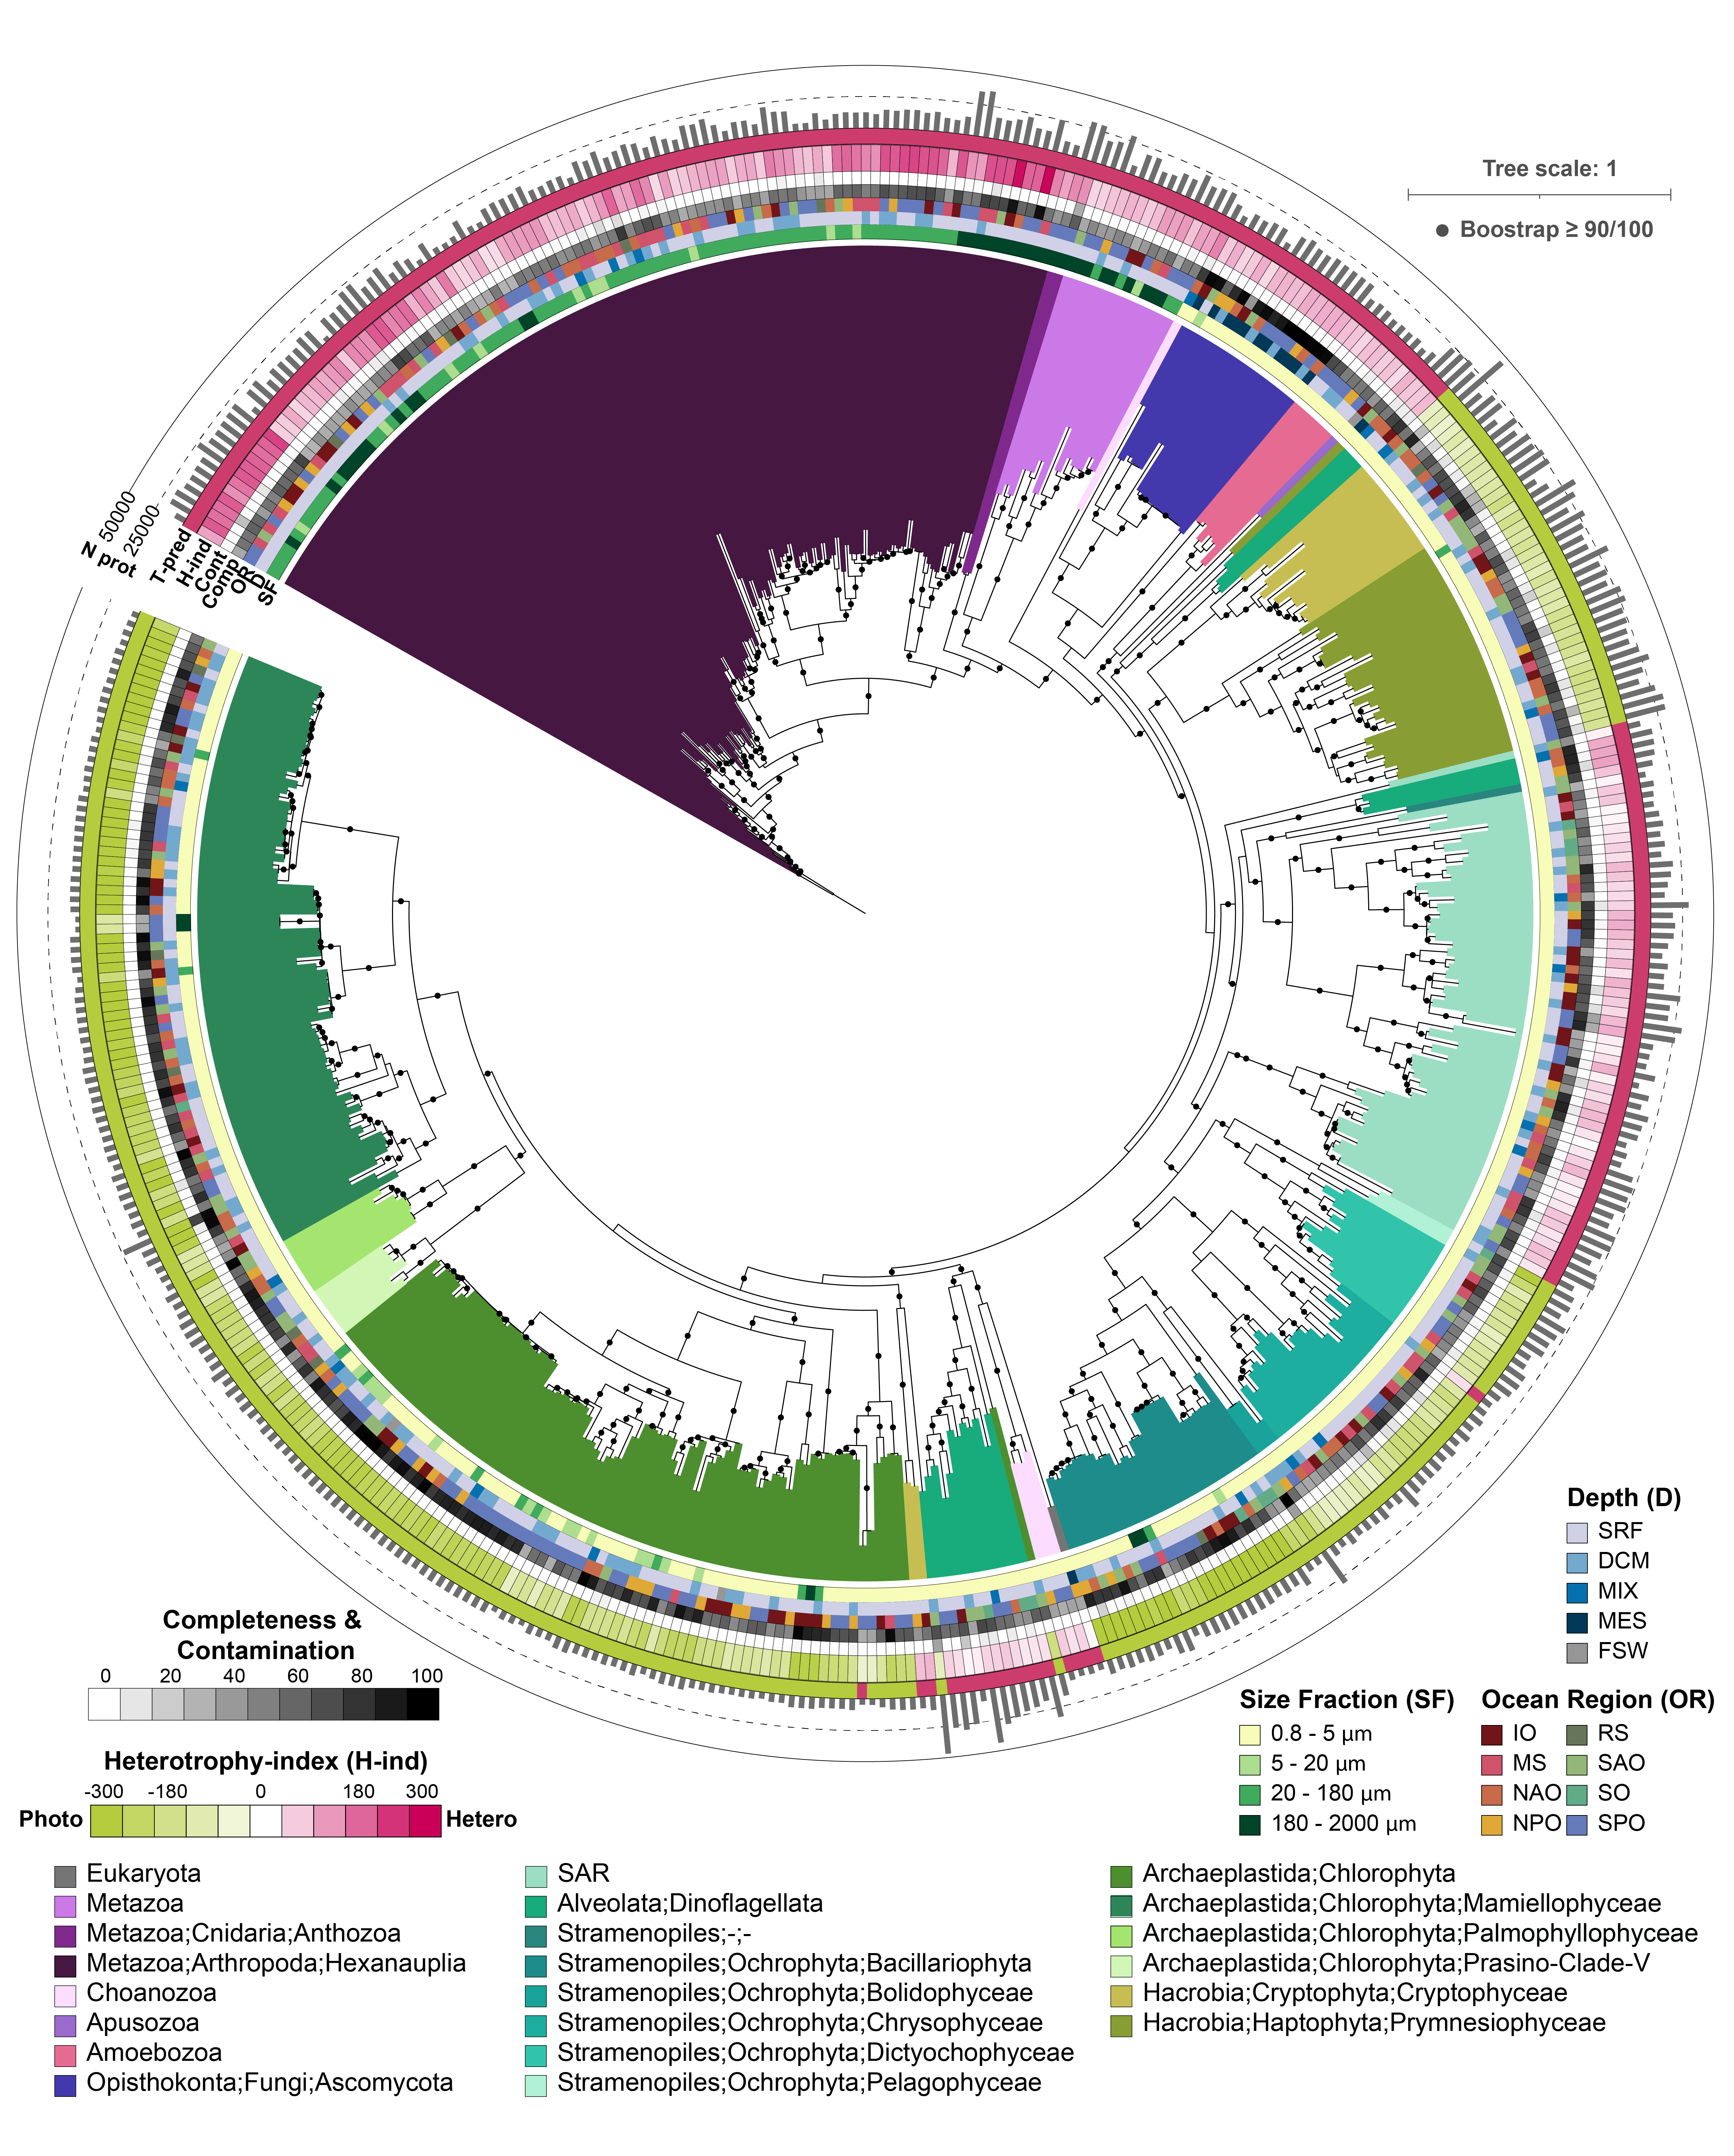
\includegraphics[width = \columnwidth]{figures/Figure3_EukPhylogeny_30Busco-v2-01.png}
    \caption{[Continued on next page.]}
    \label{fig:fig3-euk}
\end{figure}
\begin{figure}[t]
  \contcaption{\textbf{TOPAZ eukaryotic MAGs span the eukaryotic tree of life.} The maximum likelihood tree was inferred from a concatenated protein alignment of 49 proteins from the eukaryotic BUSCO gene set that were found to be commonly present across at least 75\% of the 485 TOPAZ eukaryotic MAGs that were estimated to be >30\% complete based on BUSCO ortholog presence. The MAG names were omitted but the interactive version of the tree containing the MAG names can be accessed through iTOL (\url{https://itol.embl.de/shared/halexand}). Branches (nodes) are colored based on consensus protein annotation estimated by EUKulele and MMSeqs. The Ocean Region (OR), Depth (D), and Size Fraction (SF) of the co-assembly that a MAG was isolated from is color coded as colored bars. The completeness (comp) and contamination (cont) as estimated based on BUSCO presence are depicted as a heatmap. Predicted Heterotrophy Index (H-index), which ranges from phototroph-like (-300) to heterotroph-like (300) is shown as a heatmap. The predicted trophic mode (T-pred) based on the trophy random forest classifier with heterotroph (pink) and phototroph (green), is depicted. The number of proteins predicted with EukMetaSanity are shown as a bar graph along the outermost ring. }% Continued caption
\end{figure}

The EukHeist classification pipeline identified 988 putative eukaryotic MAGs following the refinement of recovered metagenomic bins based on length ($>2.5$ Mbp) and proportion of base pairs predicted to be eukaryotic in origin by EukRep \citep{West2018Genome-reconstruction} (\ref{fig:recovered}). Protein coding regions in the eukaryotic MAGs were predicted using the EukMetaSanity pipeline \citep{EukMS}, and the likely taxonomic assignment of each bin was made with MMSeqs \citep{Steinegger2018} and EUKulele \citep{Krinos2021EUKulele} (Supplementary Table 2). Of the 988 eukaryotic MAGs recovered, 713 MAGs were estimated to be more than 10\% complete based on the presence of core eukaryotic BUSCO orthologs \citep{Simao2015BUSCO}. For the purposes of our subsequent analyses, we only consider the highly complete eukaryotic TOPAZ MAGs, or those that were greater than 30\% complete based on BUSCO ortholog presence (n=485) (\Cref{fig:fig3-euk}). 

Eukaryotic genomes are known to be both larger and have higher proportions of non-coding DNA than bacterial genomes \citep{Zhang2011practical}. On average across sequenced eukaryotic genomes, 33.1\% of genomic content codes for genes (2.6\% - 59.8\% for the 1st and 3rd quartiles) \citep{Hou_2009}, while bacterial genomes have a higher proportion of coding regions (86.9\%; 83.9\% - 89.3\%) \citep{Hou_2009}. The high-completion TOPAZ eukaryotic MAGs have an average of $73.7\% \pm 14.3\%$ gene coding regions (\Cref{fig:hq-prot-bar}). This trend of a higher proportion of coding regions was consistent across eukaryotic groups, where Haptophyta and Ochrophyta TOPAZ MAGs had an average coding region of $80.3 \pm 4.9\%$ and $78.1 \pm 6.3\%$, respectively. Genomes from cultured Haptophyta (\textit{Emiliania huxleyi} CCMP1516 with 31 Mb or 21.9\% \citep{Read2013}), and Ochrophyta (\textit{Phaeodactylum tricornutum} with 15.4 Mb or 57.3\% \citep{Bowler_2008}) had significantly lower proportions of protein coding regions within their genomes compared to TOPAZ MAGs. The lowest percentages of gene coding were within Metazoan and Fungal TOPAZ MAGs, with $52.6\pm 9.8\%$ and  $58.8 \pm 6.7\%$, respectively. As a point of comparison, the human genome is estimated to have $\approx 34$ Mb or $\approx 1.2$\% of the  genome coding for proteins \citep{humangenome}. Globally, the higher gene coding percentages for the recovered eukaryotic TOPAZ MAGs likely reflect biases caused by the use of tetranucleotide frequencies in the initial binning \citep{Kang_2019} as well as challenges inherent in the assembly of non-coding and repeat-rich regions of eukaryotic genomes. 

Phylogenetic placement of TOPAZ MAGs aligned with estimated taxonomy based on protein-consensus annotation (\Cref{fig:fig3-euk}). The recovered MAGs spanned 8 major eukaryotic supergroups: Archaeplastida (Chlorophyta), Opisthokonta (Metazoa, Choanoflagellata, and Fungi), Amoebozoa, Apusozoa, Haptista (Haptophyta), Cryptista (Cryptophyta), and the SAR supergroup (Stramenopiles, Alveolata, and Rhizaria) \citep{Burki_2020}. Eukaryotic MAGs were retrieved from all ocean regions surveyed, with the largest number of high-completion TOPAZ MAGs recovered from the South Pacific Ocean Region (SPO) (n=143) and the fewest recovered from the Southern Ocean (SO) (n=11) and Red Sea (RS) (n=12) (\Cref{fig:hq-dist}). These regional trends in MAG recovery and taxonomy aligned with the overall sequencing depth at each of these locations (Supplementary Table 1), with fewer, less diverse MAGs recovered from the SO and RS (\Cref{fig:all-dist,fig:hq-dist}).

The largest number of MAGs was recovered from the smallest size fraction ($0.8-5 \mu m$) (n=311) (\Cref{fig:fig3-euk,fig:all-dist}), and yielded the highest taxonomic diversity, including MAGs from all the major supergroups listed above (\Cref{fig:all-dist}). Chlorophyta (n=133), Ochrophyta (n=57), and taxa placed within the SAR group (Stramenopiles, Alveolata, and Rhizaria) (n=56) made up the  the largest proportion of small size fraction MAGs. Chlorophyta MAGs were smaller and had fewer predicted proteins relative to other eukaryotic MAGs, despite demonstrating comparable completeness metrics; the average Chlorophyta MAG size was 13.9 Mbp with 7525 predicted proteins (\Cref{fig:hq-prot-bar}). By contrast, Cryptophyta and Haptophyta had the largest average MAG size with 50.8 Mbp and 44.4 Mbp with an average of 23500 and 24400 predicted proteins, respectively (\Cref{fig:hq-prot-bar}). Fewer eukaryotic MAGs were recovered from the other size fractions $5-20\mu m$ (n=20), $20-180 \mu m$ (n=87), and $180-2000\mu m$ (n=39) (\Cref{fig:all-dist}), instead these larger size fractions recovered a higher total number of metazoan MAGs. Metazoan MAGs had the lowest average completeness ($50 \pm 13\%$) (\Cref{fig:all-prot-bar,fig:hq-prot-bar}); where the average size of recovered metazoan MAGs was 43.2 Mb (6.5-177Mbp), encompassing an average of 14600 proteins (\Cref{fig:hq-prot-bar}). 76 of the 123 metazoan MAGs likely belong to the  Hexanauplia (Copepoda) class; copepod genomes have been estimated to be up to 2.5 Gb with high variation (10-fold difference) across sequenced members \citep{Jorgensen_2019}. 

MAGs were also retrieved from all discrete sampling depths: surface, SRF (n=315), deep chlorophyll max, DCM (n=133), mesopelagic, MES (n=13), as well as samples with no discrete depth, MIX (n=21) and the filtered seawater controls, FSW (n=3). Notably, the FSW included 1 Chlorophyta MAG (TOPAZ\_IOF1\_E003) that was estimated to be 100\% complete with no contamination (Supplementary Table 2). 

The composition of TOPAZ MAGs from basin-scale mesopelagic co-assemblies recovered a higher percentage of fungi, relative to other depths. This is similar to other mesopelagic and bathypelagic molecular surveys, where the biomass of fungi is thought to outweigh other eukaryotes \citep{Morales_2019,Pernice_2015,Edgcomb_2010}. Further, fungal MAGs had the highest overall average completeness ($87 \pm 15\%$) (\Cref{fig:all-prot-bar,fig:hq-prot-bar}). A total of 16 highly complete fungal MAGs were also recovered, of those, 11 originated from the MES (\Cref{fig:fig3-euk,fig:hq-dist}). Putative fungal TOPAZ MAGs were recovered from the phyla Ascomycota (n=10) and Basidiomycota (n=1) and ranged in size from 12.5-47.8 Mb (\Cref{fig:hq-prot-bar}), which are within range of known average genome sizes for these groups, 36.9 and 46.5 Mb, respectively \citep{Mohanta_2015}. 

The metagenome read recruitment to these TOPAZ MAGs paralleled MAG recovery, where metazoan MAGs dominated the larger size fractions ($20-180 \mu m$ and $180-2000 \mu m$) across both the surface and DCM for all stations, and Chlorophyta MAGs were dominant across most of the small size fraction stations ($0.8-5 \mu m$) (\Cref{fig:map}). A notable exception are the stations from the Southern Ocean, where Haptophyta and Ochrophyta were most abundant in all size fractions. Compared to the samples from the photic zone, SRF and DCM, the average recruitment of reads from the MES was far lower ($24500 \pm 34450$ average CPM in the MES compared to $131000 \pm 104000 $ and $136000 \pm 85000$ for the SRF and DCM, respectively (\Cref{fig:map}). This suggests that the mesopelagic have high variability across communities \citep{Pernice_2015} and that we did not fully capture the eukaryotic MAGs that adequately describe all surveyed communities. Alternatively, this might suggest that the communities sampled were dominated by prokaryotic biomass \citep{Pernice_2014}.  


\subsection*{Trophic mode can be predicted from MAG gene content}

\begin{figure}[h!]    
    \centering
    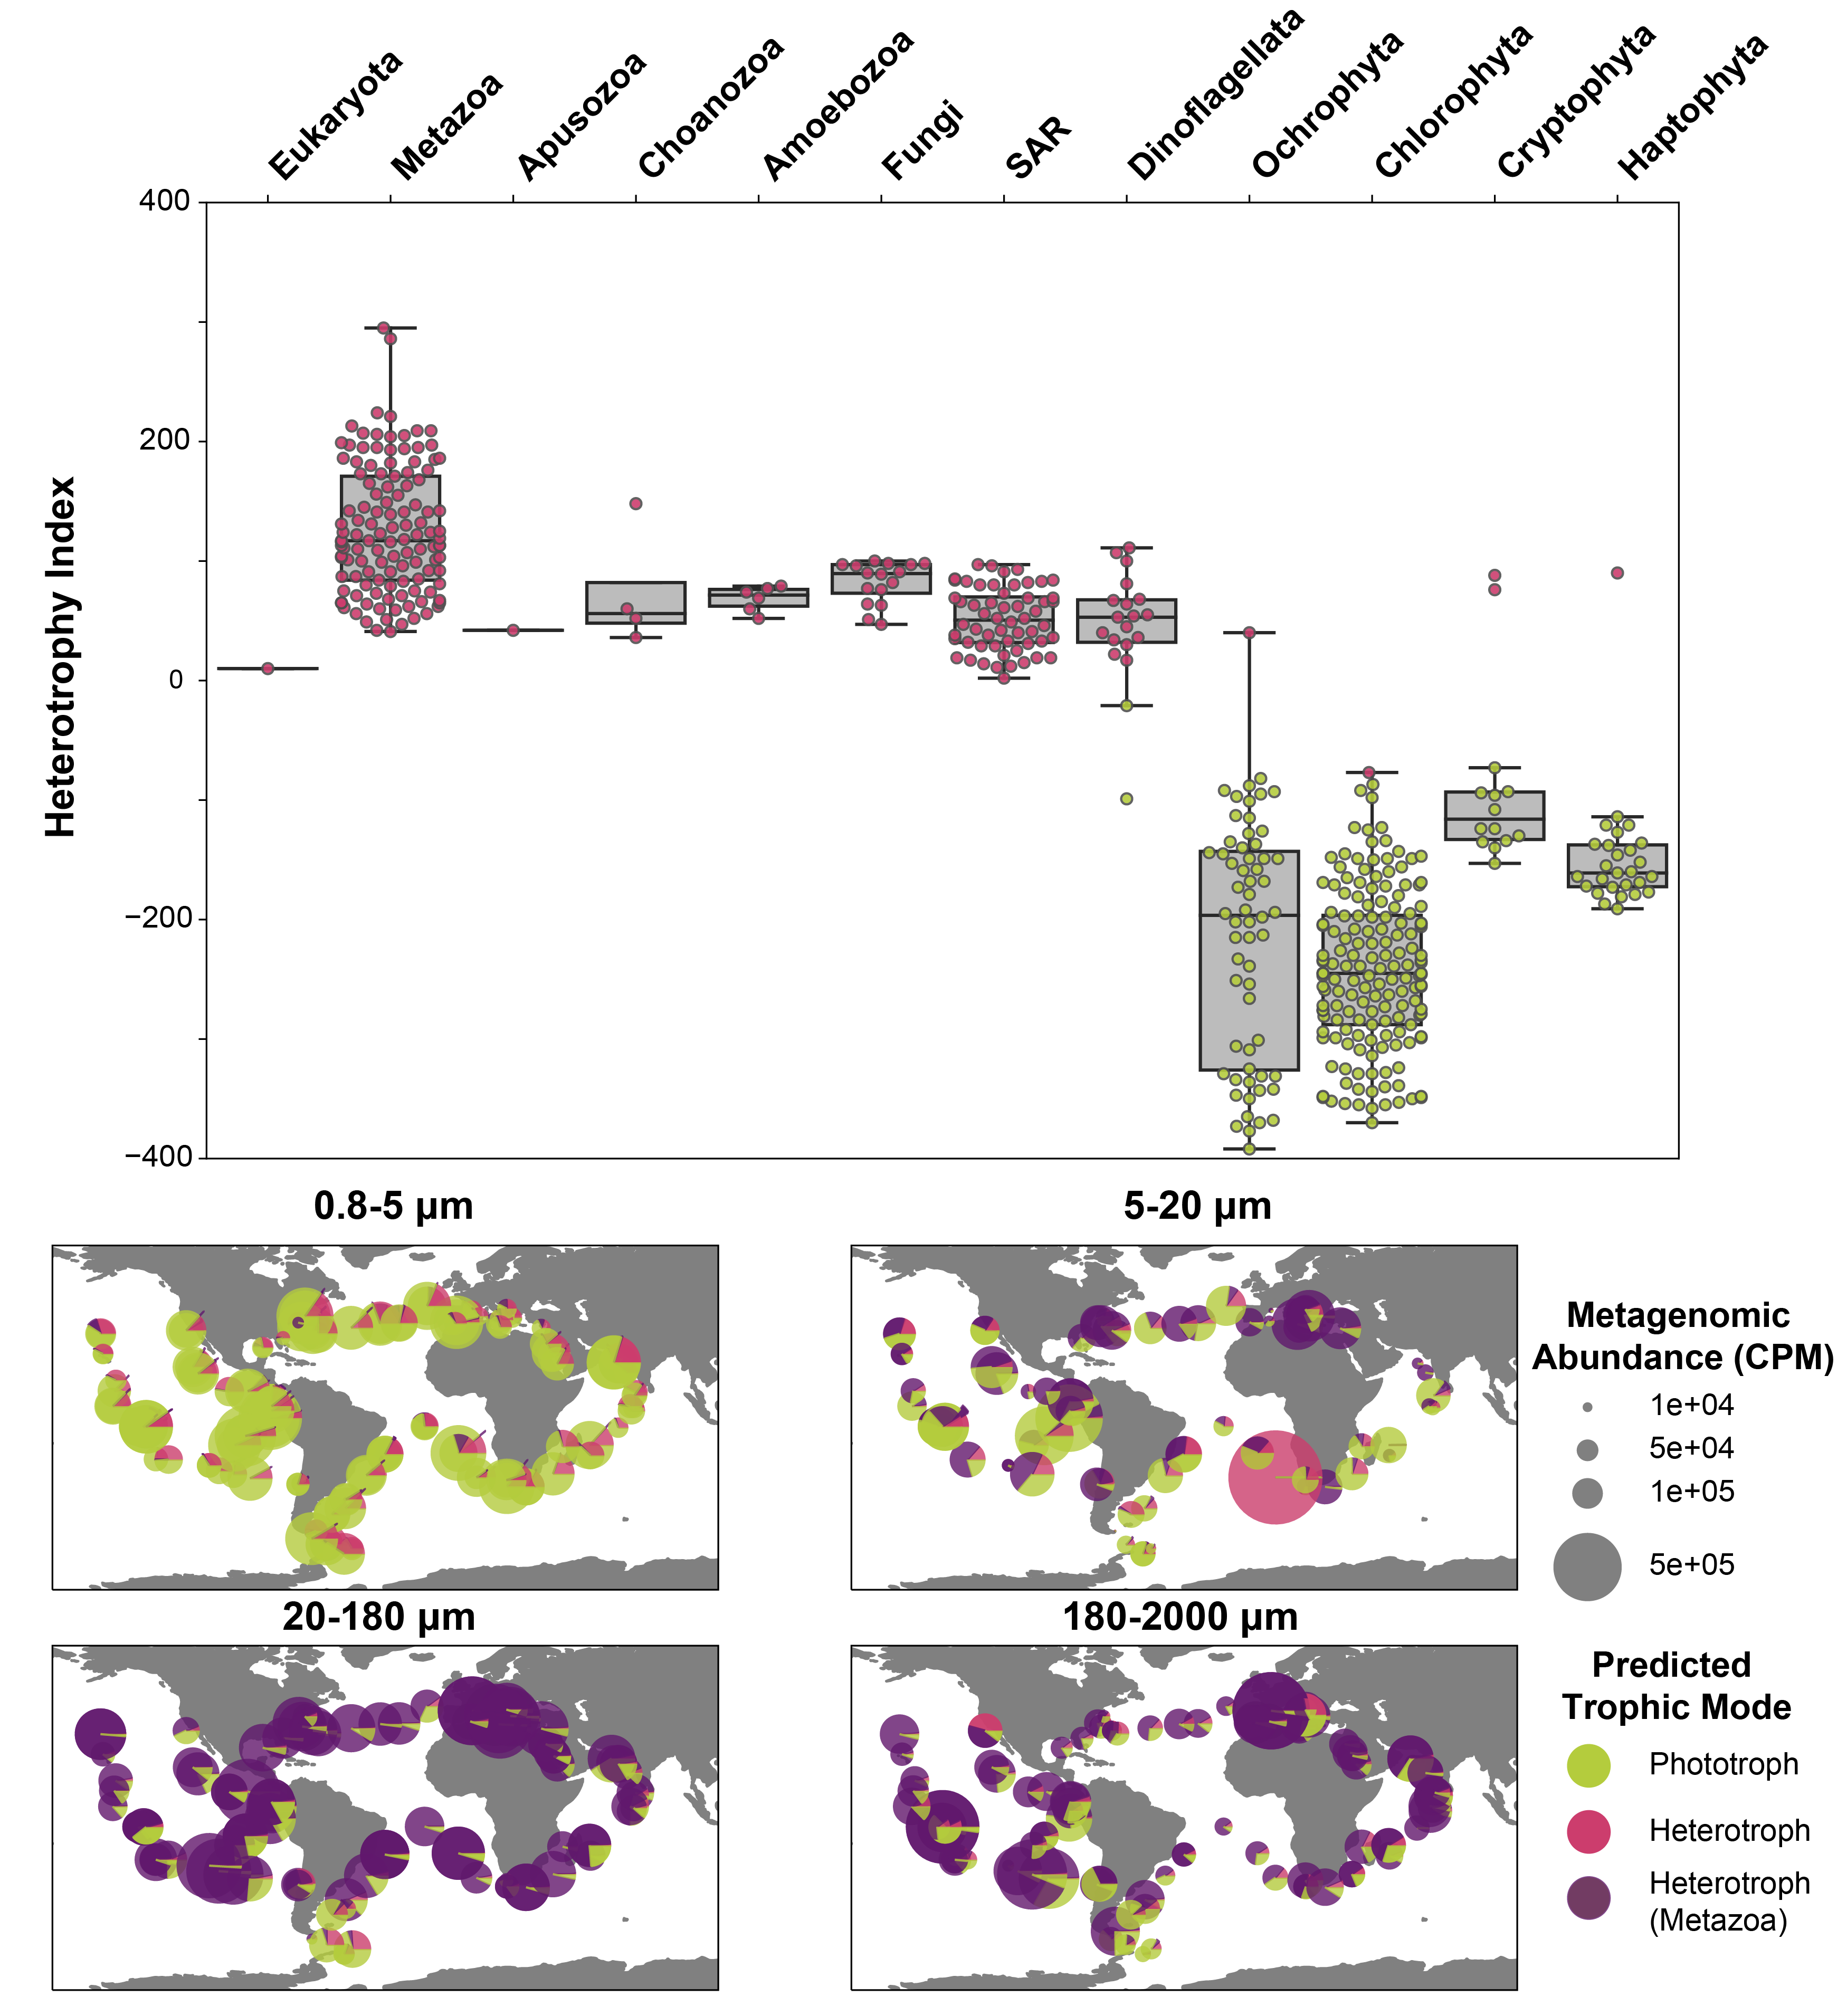
\includegraphics[width = 0.9\columnwidth]{figures/Figure4_Trophic_Mode_v2-01.png}
    \caption{\textbf{Estimated trophic status of TOPAZ eukaryotic MAGs.} (Top) Trophic status was predicted for each high-completion TOPAZ eukaryotic MAG using a Random Forest model trained on the presence and absence of KEGG orthologs and is shown as a color (green, phototroph, pink, heterotroph). The Heterotrophy Index (H-index) (\cref{eq:hind}) for each MAG is plotted with a box plot showing the range of the H-index for each higher level group. (Bottom) The relative distribution and abundance of Phototroph (green), non-Metazoan Heterotroph (Pink), and Metazoan Heterotroph (Purple) is depicted across all surface samples. Plots are subdivided by size classes. }
    \label{fig:fig4-trophy}
\end{figure}

Eukaryotic microbes can exhibit a diversity of functional traits and trophic strategies in the marine environment \citep{Worden2015} \citep{Caron2011Marine}; including, phototrophy, heterotrophy, and mixotrophy. Phototrophic protists are responsible for a significant fraction of the organic carbon synthesis via primary production; these phototrophs dominate the microbial biomass and diversity in the sunlit layer of the oceans \citep{Worden2015,de_Vargas_2015}. Phagotrophic protists (heterotrophs), which ingest bacteria, archaea, and smaller eukaryotes, and parasitic protists are known to account for a large percentage of mortality in food webs \citep{Sherr_2002, Caron2011Marine, Worden2015}. Protists are also capable of mixed nutrition (mixotrophy), where a single-cell exhibits a combination of phototrophy and heterotrophy \citep{Stoecker_2017}. Typically, the identification of trophic mode has relied upon direct observations of isolates within an lab setting, with more recent efforts including transcriptional profiling as a means of assessing trophic strategy \citep{Keeling2014, Liu_2016}. Scaling up these culture-based observations to environmentally-relevant settings \citep{Alexander2015a, hu2018,Gong_2016} has been an important advance in the field for exploring complex communities without cultivation. An outcome from these studies has been the realization that trophic strategies are not governed by single genes \citep{Labarre_2020}; in reality, trophic strategy will be shaped by an organisms' physiological potential and environmental setting. Therefore larger genomic and transcriptomic efforts to predict or characterize presumed trophic strategies among mixed microbial communities will greatly contribute to our understanding of the role that microorganisms play in global biogeochemical cycles, by enabling the observation of functional traits and strategies \textit{in situ}. 

Large scale meta'omic results, such the TOPAZ MAGs recovered here, can be leveraged alongside presently available reference data to enable the prediction of biological traits (such as trophic mode) without \textit{a priori} information. Machine learning (ML) applications can be implemented to access the potential of these large datasets. ML approaches have been recently shown to be capable of accurate functional prediction and cell type annotation using genetic input, in particular for cancer cell prediction \citep{shipp2002diffuse,bashiri2017improving,tabl2019machine}, and functional gene and phenotype prediction in plants \citep{mahood2020machine}. Recently, these approaches have been applied to culture and environmental transcriptomic data to predict trophic mode using currently available trophy annotations \citep{lambert2021dynamic, burns2018gene,Jimenez_2021}. Here, we apply an independent machine learning model to the eukaryotic TOPAZ MAGs to predict each organisms' capacity for various metabolisms.

Using a reference set built from protistan transcriptomic data, we predicted the trophic mode of the highly complete TOPAZ MAGs using machine learning and direct estimation via presence of important KEGG pathways (\cref{eq:hind}). As the gradient of trophic mode among protists is not strictly categorical, we calculated a Heterotrophy Index (H-index) that places the TOPAZ MAGs on a scale of highly phototrophic (negative values) to highly heterotrophic (positive values) (\Cref{fig:fig3-euk,fig:fig4-trophy}). Thus, for all sufficiently complete ($\geq30\%$) TOPAZ MAGs we have predicted both a gross trophic category (heterotrophic ($n=227$), mixotrophic ($n=0$), or phototrophic ($n=258$) as well as the quantitative extent of heterotrophy (H-index, \cref{eq:hind}). Broadly, the trophic predictions aligned well with the putative taxonomy of each MAG (\Cref{fig:fig3-euk,fig:fig4-trophy}). For example, TOPAZ MAGs that had taxonomic annotation of well known heterotrophic lineages (Metazoa, Fungi),  were predicted as heterotrophs based on our model.  Further, our data-driven trophic mode predictions correlate well with an independent model designed to identify the presence of photosynthetic machinery and capacity for phagotrophy \citep{burns2018gene} (\Cref{fig:mag-burns,fig:mmetsp-burns}). 

Despite evidence that many lineages recovered include known mixotrophs, no TOPAZ MAGs were identified as mixotrophic using this approach. However, the utility of the H-index enables us to still consider mixotrophic-capable MAGs. We explore the likely reasons for this more deeply in the \Cref{limitations}, but one potential explanation is that MAG recovery targets the genomic content of a eukaryotic lineage and the evolutionary history of phototrophy and heterotrophy is complicated and varies with respect to species \citep{Flynn_2019}. Therefore, the genetic composition of MAGs may reflect encoded metabolisms that are not necessarily exhibited \textit{in situ}. Additionally, mixotrophy is not a singular trait, but rather a spectrum of metabolic abilities that are largely driven by the microorganisms' nutritional needs and surrounding environment. Continued culturing combined with large-scale 'omic efforts will continue to improve such ML models focused on complex traits and ultimately our ability to predict trophic mode. We suggest that the integration of metagenomic and metatranscriptomic datasets might better reflect the active strategies being used. 

\subsection*{Ecological niches of heterotrophic and phototrophic Stramenopiles using metatranscriptomic evidence}

A total of 24 high-completion TOPAZ eukaryotic MAGs were subset as a case study to explore the utility of pairing metatranscriptome data with MAG results to characterize the ecological context of less resolved protistan lineages. Selected MAGs included 11 taxonomically-assigned as \textit{Dictyochophyceae} (silicoflagellates), which were putatively classified as phototrophs with our trophic model (\Cref{fig:fig4-trophy}), and 13 MAGs within a phylogenetically-related stramenopile clade and classified as heterotrophs (\Cref{fig:fig3-euk,fig:fig5-dicty} a). 


\begin{figure}[h!]    
    \centering
    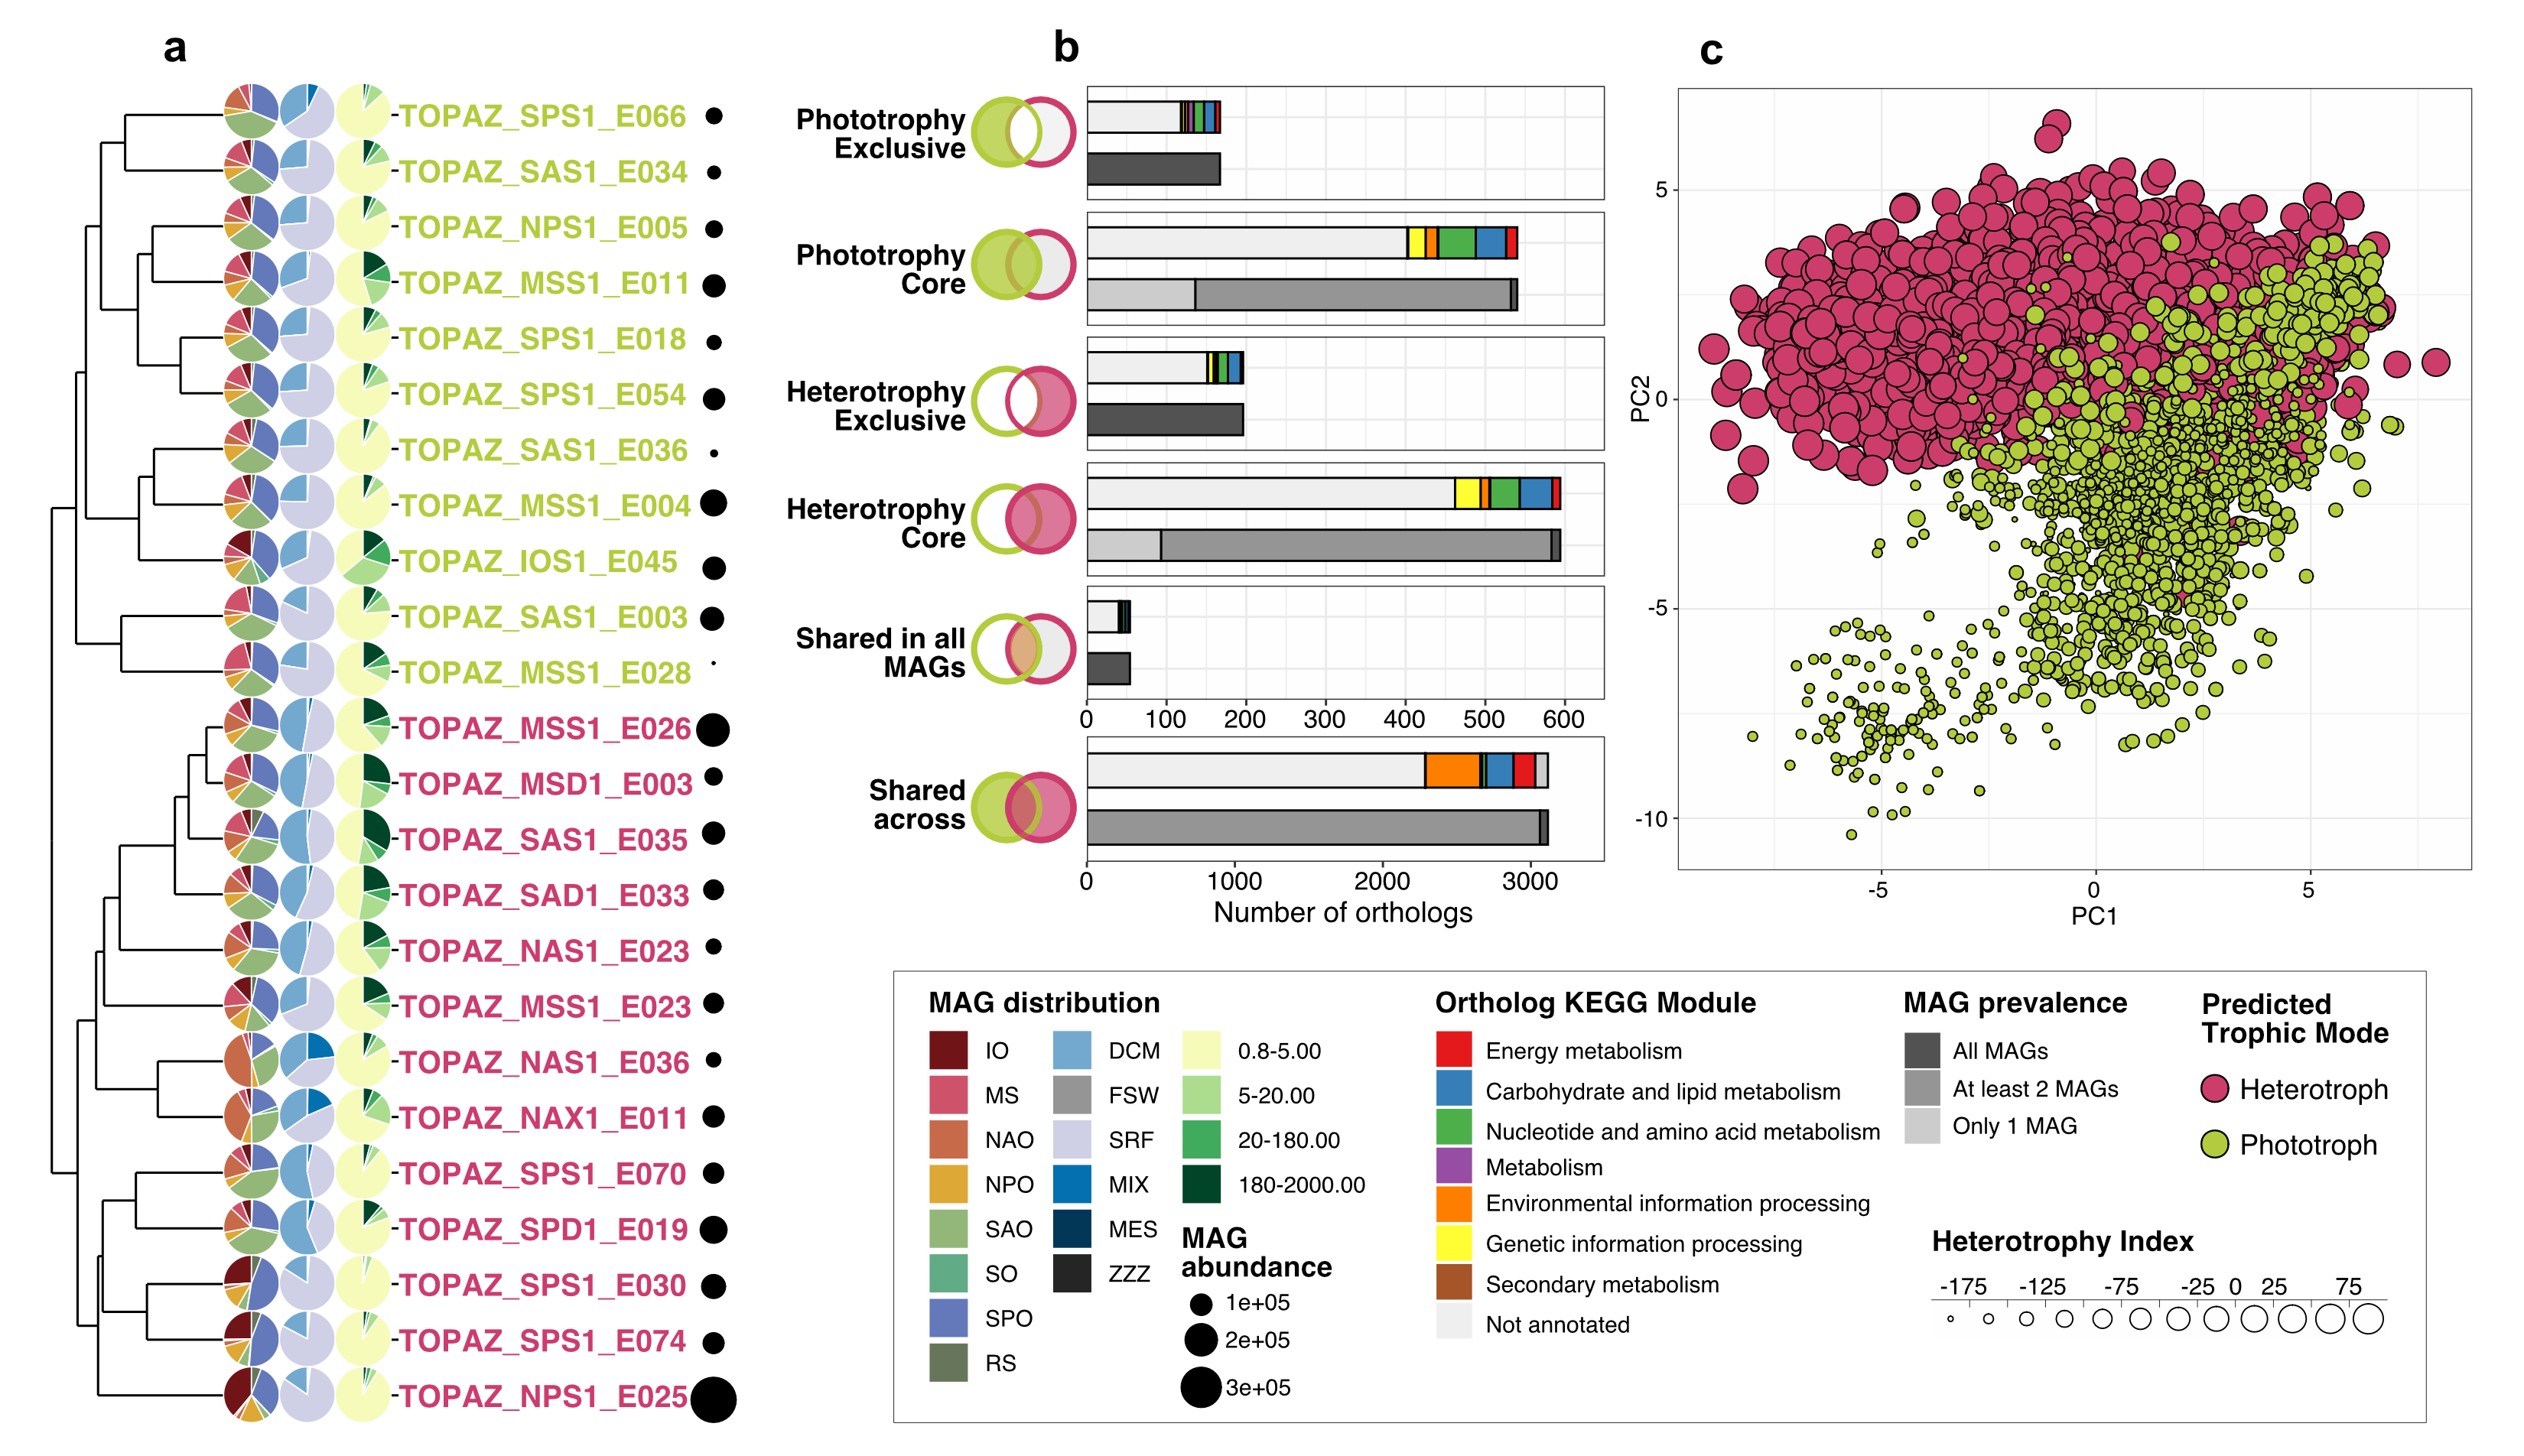
\includegraphics[width = \columnwidth]{figures/Figure5-panel-plot-stramenopile-H.png}
    \caption{ \textbf{Dictyochophyceae and stramenopile MAGs} A subset of 24 highly-complete TOPAZ MAGs taxonomically classified as stramenopiles and \textit{Dictyochophyceae}. (a) Cluster dendrogram derived from the presence or absence of orthologs grouped MAGs by predicted trophic mode (green indicates phototrophy and pink indicates heterotrophy). Pie charts to the left of each TOPAZ MAG name indicate the relative CPM abundance of each MAG for (left to right pies) ocean region, depth sampled, and size fraction. Bubble plots to the right of each TOPAZ MAG name indicate the total MAG CPM abundance. (b) Summary of shared and unique orthologs based on occurrence in phototrophy- and heterotrophy-predicted TOPAZ MAGs. Venn diagrams indicate category of orthologs shown in each panel, while panels report the KEGG module and prevalence among MAGs in each category (bar plot). (c) Principle component analysis derived from metatranscriptome reads, from the surface and smallest size fraction, mapped to shared orthologs (Shared in all MAGs in (b)) among all 24 MAGs. Symbol size designates Heterotrophy Index, while symbol color denotes predicted trophic mode. 
    }
    \label{fig:fig5-dicty}
\end{figure}
All 24 MAGs had a cosmopolitan distribution primarily originating from surface samples from the smallest size fraction, but some individual MAGs had relatively higher CPM abundances suggesting environmental selection based on oceanographic region (\Cref{fig:fig5-dicty}a, \Cref{fig:dictyocho-SAR-map}, \Cref{fig:dictyocho-SAR-heatmap}). The biogeography of the \textit{Dictyochophyceae} aligned with existing literature, where \textit{Dictyochophyceae} are globally distributed and typically found in the euphotic layer of the world ocean \citep{vaulot2008fmr, obiol2020mer, massana2011arm}. Global sampling efforts have also recovered genetic signatures of \textit{Dictyochophyceae} as a prominent, but not abundant, member of the Stramenopile group that does not demonstrate remarkable seasonality \citep{giner2019me, obiol2020mer}. While grazing on bacteria and picocyanobacteria has been observed within mixotrophic \textit{Dictyochophyceae}, previous work to quantify grazing rates were unsuccessful to due to the low cell abundance \citep{unrein2014ij}. Therefore, metagenomic and metatranscriptomic datasets, such as the recovered TOPAZ MAGs, are well suited to illuminate the biogeography and functional potential of the \textit{Dictyochophyceae}. \textit{Dictyochophyceae} and heterotrophic Stramenopiles have previously been reported in analyses of the \textit{Tara} Oceans data \citep{Carradec2018global, pierellakarlusich2020arms, vorobev2020gra, sieracki2019sr}.

Results enabled both targeted and untargeted approaches to investigate the physiology of SAR TOPAZ MAGs. First, we assessed ortholog co-occurrence across the MAGs to identify genes that were present only among the phototrophy-predicted \textit{Dictyochophyceae} MAGs (Phototrophy Exclusive; \Cref{fig:fig5-dicty}b). Genes deemed Phototrophy Exclusive (\Cref{fig:fig5-dicty}b) were related to chlorophyll biosynthesis (Por; protochlorophyllide reductase), enzymes integral to the pentose phosphate pathways, and acyltransferases and carboxylases, which are involved in \textit{de novo} fatty acid biosynthesis functions (e.g., ACACA; acetyl-CoA carboxylase biotin, ACSS; acetyl-coA synthetase). Inversely, genes detected only within putative stramenopile MAGs classified as heterotrophs (\textit{i.e.}, Heterotrophy Exclusive; \Cref{fig:fig5-dicty} b) included enzymes integral for the breakdown of large sugar molecules such as glycosaminoglycans (\textit{e.g.}, IDUA; L-iduronidase, UDP-glucose:O-linked fucose beta-1,3-glucosyltransferase, NAGLU; alpha N acetylglucosaminidase, IDS; iduronate-2sulfatase, and GALC; galactosylceramidases). Enzymes associated with glycosaminoglycan metabolism may be associated with cell adhesion or the intracellular re-processing of glycosaminoglycan; the latter of which may be a genetic attribute for more heterotrophic lifestyles. By isolating the presence and absence of specific genes across MAGs with varied predicted trophic modes, we can identify sets of genes that may be indicative of a species' ecological role. 

Ordination results based on transcripts shared across all 24 MAGs (\Cref{fig:fig5-dicty} c; based on ‘Shared in all MAGs’ in \Cref{fig:fig5-dicty}b) clustered by H-index and TOPAZ MAG identity (\Cref{fig:dictyocho-SAR-PCA-mag}). While there was some overlap among MAGs predicted to be heterotrophic versus phototrophic, trends dictating the PCA results appeared to be driven primarily by the trophic mode of individual MAGs, rather than region sampled (\Cref{fig:fig5-dicty} c, \Cref{fig:dictyocho-SAR-PCA-mag}). Further, ordination results resembled previously observed trends from transcript-based efforts to separate phototrophic, mixotrophic, and heterotrophic protistan species from cultivation \citep{koid2014po, beisser2017p} and the environment \citep{hu2018}. Results from the mapped metatranscriptome reads revealed populations to exhibit more heterotrophic or phototrophic traits depending on the environment (\Cref{fig:dictyocho-SAR-pho-lolli}, \Cref{fig:dictyocho-SAR-het-lolli}). For instance, among the \textit{Dictyochophyceae}-predicted MAGs variable phototrophic versus heterotrophic relative abundances may reflect a mixotrophic-capable population responding to the environment (\Cref{fig:dictyocho-SAR-pho-lolli}). The 13 MAGs classified as heterotrophic (ML model in this study) were phylogenetically similar to  other Stramenopiles (\Cref{fig:fig5-dicty} b \& \Cref{fig:fig3-euk}) and H-indices reported for each MAG aligned with what was seen in the metatranscriptome signal, where MAGs with the highest heterotrophy scores (e.g., TOPAZ\_SAS1\_E035 and TOPAZ\_NAX\_E011; \Cref{fig:dictyocho-SAR-PCA-mag}) had higher CPM associated with heterotrophic traits in all samples (\Cref{fig:dictyocho-SAR-het-lolli}). While the identity of the \textit{Dictyochophyceae} MAGs was further supported by phylogenetic similarity with other \textit{Dictyochophyceae} MAGs and single-cell genome-informed MAGs (\Cref{fig:dictyocho-SAR-tree-itol}), the taxonomic identity of the presumed heterotrophic Stramenopile TOPAZ MAGs was less resolved. While we cannot confidently annotate beyond the taxonomic classification of 'SAR', these MAGs were distinct from those in culture and likely include a mixotrophic-capable group of protists distinct from the MArine STramenopiles (MAST; \Cref{fig:dictyocho-SAR-tree-itol}). These findings demonstrate the value of large untargeted genetic approaches to gain insight into the \textit{in situ} metabolisms of less explored branches of the eukaryotic tree of life. Paired metagenomic and metatranscriptome results, alongside the environmental context provided by a large-scale global sampling effort, and the predicted nutritional strategies we can gain a more comprehensive understanding of protists in our oceans.


\subsection*{TOPAZ prokaryotic MAGs distinct from previous marine MAG recovery efforts}

\begin{figure}[h!]    
    \centering
    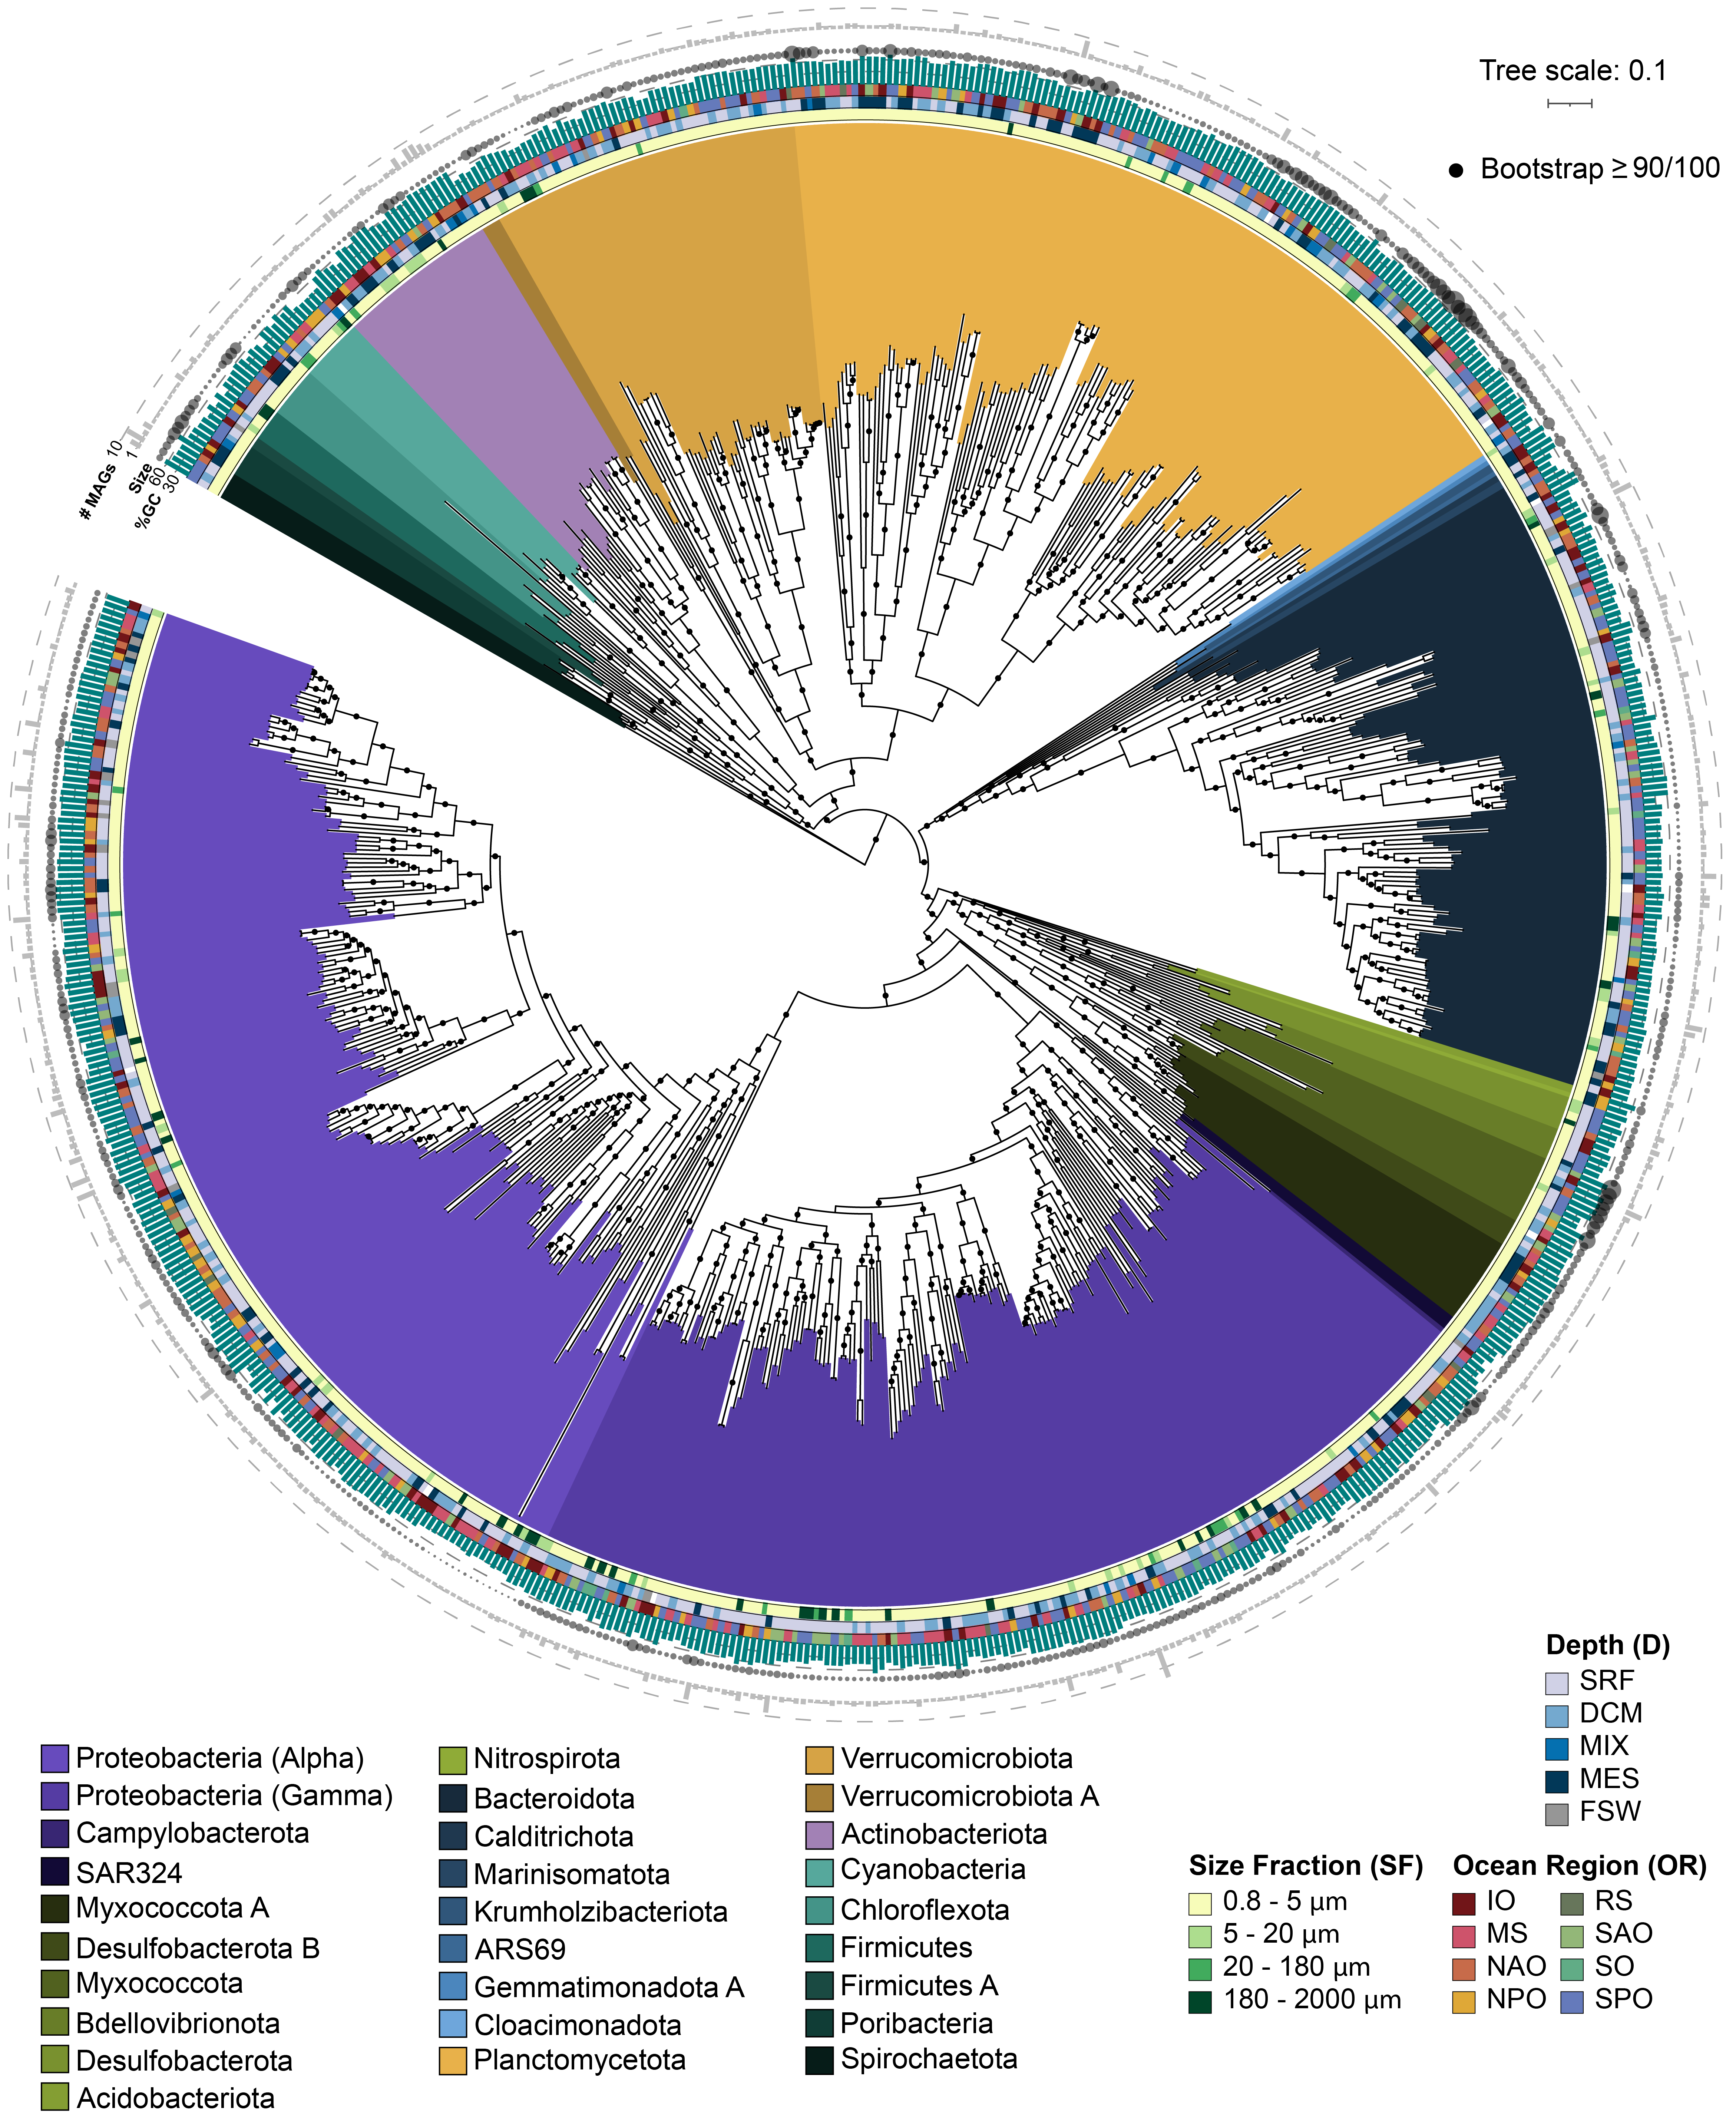
\includegraphics[width =\columnwidth]{figures/Figure1-Bacterial-phylogeny.png}
    \caption{[Continued on next page.]}
    \label{fig:fig1-prokaryotes}
\end{figure}
\begin{figure}[t]
    \contcaption{\textbf{Diversity of the high-quality non-redundant bacterial TOPAZ MAGs.} The approximately-maximum-likelihood phylogenetic tree was inferred form a concatenated protein alignment of 75 proteins using FastTree and GToTree workflow. The MAG names were omitted but the interactive version of the tree containing the MAG names can be accessed through iTOL (\url{https://itol.embl.de/shared/halexand}). Branches (nodes) are colored based on taxonomic annotations estimated by GTDBtk. The Ocean Region (OR), Size Fraction (SF), and Depth (D) of the co-assembly that a MAG was isolated from is color coded as colored bars. The GC (\%) content is shown as a bar graph (in green), the genome size as bubble plot (the estimated size of the smallest genome included in this tree is 1.00Mbp and the largest is 13.24Mbp) and the number of MAGs in each genomic cluster (of 99 or higher \%ANI) as a bar plot (in grey)}
\end{figure}

The vast majority of the retrieved prokaryotic MAGs belonged to Bacteria. High-quality non-redundant TOPAZ (HQ-NR-TOPAZ) MAGs were comprised of 711 bacterial and 5 archaeal MAGs belonging to 30 different phyla (\Cref{fig:fig1-prokaryotes} and Supplementary Table 4); an additional 15 phyla were recovered in the medium quality (MQ) MAGs. Of the 716 HQ-NR-TOPAZ MAGs, 507 were unique based on a 99\% ANI comparison threshold with MAGs generated from previous binning efforts from \textit{Tara} Oceans metagenomic data, including \citet{Delmont2018Nitrogen-fixing} (TARA), \citet{Tully2018reconstruction} (TOBG), and \citet{Parks2017Recovery} (UBA) (\Cref{fig:fig1-prokaryotes}). The phylogenetic diversity captured by the TOPAZ MAGs was quantified by a comparison to a "neutral" reference set of genomes; these neutral references approximate the state of marine microbial genomes, dominated by isolate genomes, previous to the incorporation of the \textit{Tara} Oceans-derived MAGs. Relative to the neutral genomic references, the entire TOPAZ NR (includes both HQ and MQ) set represented a 42.8\% phylogenetic gain (as measured by additional branch length contributed by a set of data) and 59.9\% phylogenetic diversity (as measured by the total branch length spanned by a set of taxa), as compared to efforts focused solely on the smaller size fractions such as TARA and UBA, which had a smaller degree of gain (31.0\% and 25.8\%, respectively) and diversity (44.4\% and 40.5\%, respectively). An inclusive tree containing the neutral reference and all \textit{Tara} Oceans MAGs (TOBG + UBA + TARA + TOPAZ), the TOPAZ NR MAGs represented 14.4\% of the phylogenetic gain and 44.7\% phylogenetic diversity, suggesting that the TOPAZ MAGs offer the largest increase in phylogenetic novelty when compared to MAGs reconstructed from the metagenomes of the smaller size fractions ($<5.00 \mu m$). The TOPAZ MAGs primarily originated from the larger \textit{Tara} Ocean size fraction samples, and thus include a higher proportion of more complex host- and particle-associated bacterial communities. The novelty of the HQ- and MQ-NR-TOPAZ MAGs here, suggests that these particle-associated MAGs are overlooked and current genome databases are largely skewed towards free-living bacteria.

%Copiotrophs are predicted to have
%higher copy numbers of rRNA operons and tRNA genes, because higher numbers of these
%genes increase their maximum overall transcription rates, helping maintain higher abundances
%of ribosomes

To confirm the hypothesis that the prokaryotic TOPAZ MAGs included particle-associated members, we examined the genomic features of several selected groups that were well-recovered here and in single-cell amplified genomic datasets (i.e., GORG) \citep{Pachiadaki_2019}.  To avoid potential biases related to completeness and contamination of the genomes, only the HQ-NR MAGs were compared to the GORG SAGs, and analyses were limited to groups with sufficient representation within both datasets (Bacteriodota, Cyanobacteria, and Proteobacteria). For these well represented groups, the average GC\% and estimated genome size of the TOPAZ MAGs were significantly higher than the ones typically reported in free-living marine bacteria \citep{Dufresne_2005, Swan_2013, Luo_2015} and those observed within the GORG dataset \citep{Pachiadaki_2019}. TOPAZ MAGs were found to encode more tRNAs on average per genome than GORG (39.5 vs 30). Additionally, Carbohydrate-Active Enzymes (CAZy) and peptidases were enriched within the TOPAZ MAGs relative to GORG (\Cref{fig:fig6-prokfunc}).  Larger genomes have been considered diagnostic for a copiotrophic lifestyle in bacteria \citep{Okie_2020}, since the more extended and flexible gene repertoire can facilitate substrate catabolism in organic rich niches such as particles. Genomes of copiotrophs are also commonly found to have higher copy numbers of genes associated with replication and protein biosynthesis such as tRNAs and rRNAs \citep{Rocha_2004} which facilitate higher growth rates. In contrast, the streamlined genomes of SAR11 and other groups that have free-living oligotrophic lifestyles require fewer resources to maintain and replicate their genomes and have higher carbon-use efficiency \citep{Giovannoni_2014}. Similarly, G and C have higher energy cost of production and more limited intracellular availability compared to A and T \citep{Moore_2013, Luo_2015}. The genomic trends observed support our findings that TOPAZ MAGs represent both particle associated and free-living microbes, and are relatively enriched for copiotrophic microbes.

\begin{table}[]
\caption{\textbf{Phylogenetic diversity and gain of various MAGs originating from \textit{Tara} Oceans.} Phylogenetic diversity and gain of prokaryotic MAGs was assessed for this study (TOPAZ), TOBG \citep{Tully2018reconstruction}, UBA \citep{Parks2017Recovery}, and TARA \citep{Delmont2018Nitrogen-fixing} relative to each other as well as a "Neutral" tree comprised of relevant marine bacteria.}
\centering
\begin{tabular}{|
>{\columncolor[HTML]{EFEFEF}}c |c|c|c|c|}
\hline
{\color[HTML]{000000} \textbf{Base tree}}                  & \cellcolor[HTML]{EFEFEF}\textbf{\begin{tabular}[c]{@{}c@{}}MAGs \\ of interest\end{tabular}} & \cellcolor[HTML]{EFEFEF}\textbf{\begin{tabular}[c]{@{}c@{}}No. of \\ MAGs\end{tabular}} & \cellcolor[HTML]{EFEFEF}\textbf{\begin{tabular}[c]{@{}c@{}}Phylogenetic \\ diversity* \end{tabular}} & \cellcolor[HTML]{EFEFEF}\textbf{\begin{tabular}[c]{@{}c@{}}Phylogenetic \\ gain\textdegree \end{tabular}} \\ \hline
{\color[HTML]{000000} \textbf{Neutral}} & TOPAZ (MQ, NR) & 1,571            & 59.9\%  & 42.8\%            \\ \hline
{\color[HTML]{000000} \textbf{Neutral}} & TOPAZ (HQ, NR) & 634              & 41.6\%  & 25.8\%            \\ \hline
{\color[HTML]{000000} \textbf{Neutral}} &   TOBG     & 1,974            & 61.3\%  & 46.7\%            \\ \hline
{\color[HTML]{000000} \textbf{Neutral}} & UBA            & 1,052            & 40.5\%  & 25.8\%            \\ \hline
{\color[HTML]{000000} \textbf{Neutral}} & TARA           & 722              & 44.4\%  & 31.0\%            \\ \hline
{\color[HTML]{000000} \textbf{Neutral}} & TOBG + UBA + TARA               & 3,750            & 66.6\%  & 51.8\%            \\ \hline
{\color[HTML]{000000} \textbf{\begin{tabular}[c]{@{}c@{}}Neutral + \textit{Tara} \\ Oceans MAGs\textsuperscript{HQ}\end{tabular}}}  & TOPAZ (HQ, NR) & 634              & 26.1\%  & 6.2\%             \\ \hline
{\color[HTML]{000000} \textbf{\begin{tabular}[c]{@{}c@{}}Neutral + \textit{Tara} \\ Oceans MAGs\textsuperscript{MQ}\end{tabular}}}  & TOPAZ (MQ, NR) & 1,572            & 44.7\%  & 14.4\%            \\ \hline
{\color[HTML]{000000} \textbf{\begin{tabular}[c]{@{}c@{}}Neutral + \textit{Tara} \\ Oceans MAGs\textsuperscript{MQ}\end{tabular}}} & TOBG           & 1,977            & 48.5\%  & 11.1\%            \\ \hline
{\color[HTML]{000000} \textbf{\begin{tabular}[c]{@{}c@{}}Neutral + \textit{Tara} \\ Oceans MAGs\textsuperscript{MQ}\end{tabular}}}  & UBA            & 1,055            & 23.8\%  & 1.6\%             \\ \hline
{\color[HTML]{000000} \textbf{\begin{tabular}[c]{@{}c@{}}Neutral + \textit{Tara} \\ Oceans MAGs\textsuperscript{MQ}\end{tabular}}} & TARA           & 722              & 28.0\%  & 3.4\%             \\ \hline
\multicolumn{5}{l}{\begin{tabular}[c]{@{}l@{}}\textbf{*} total branch length spanned by a set of taxa\\ \textbf{\textdegree} additional branch length contributed by a set of taxa\\ \textsuperscript{HQ} includes Neutral, TOBG, UBA, TARA, and TOPAZ HQ, NR MAGs\\ \textsuperscript{MQ} includes Neutral, TOBG, UBA, TARA, and TOPAZ MQ, NR MAGs
\end{tabular}}                
\end{tabular}
\label{tab:mags}
\end{table}

\subsection*{Environmental factors structure TOPAZ MAG co-occurrence }

\begin{figure}[h!]    %Place holder figure for right now. 
    \centering
    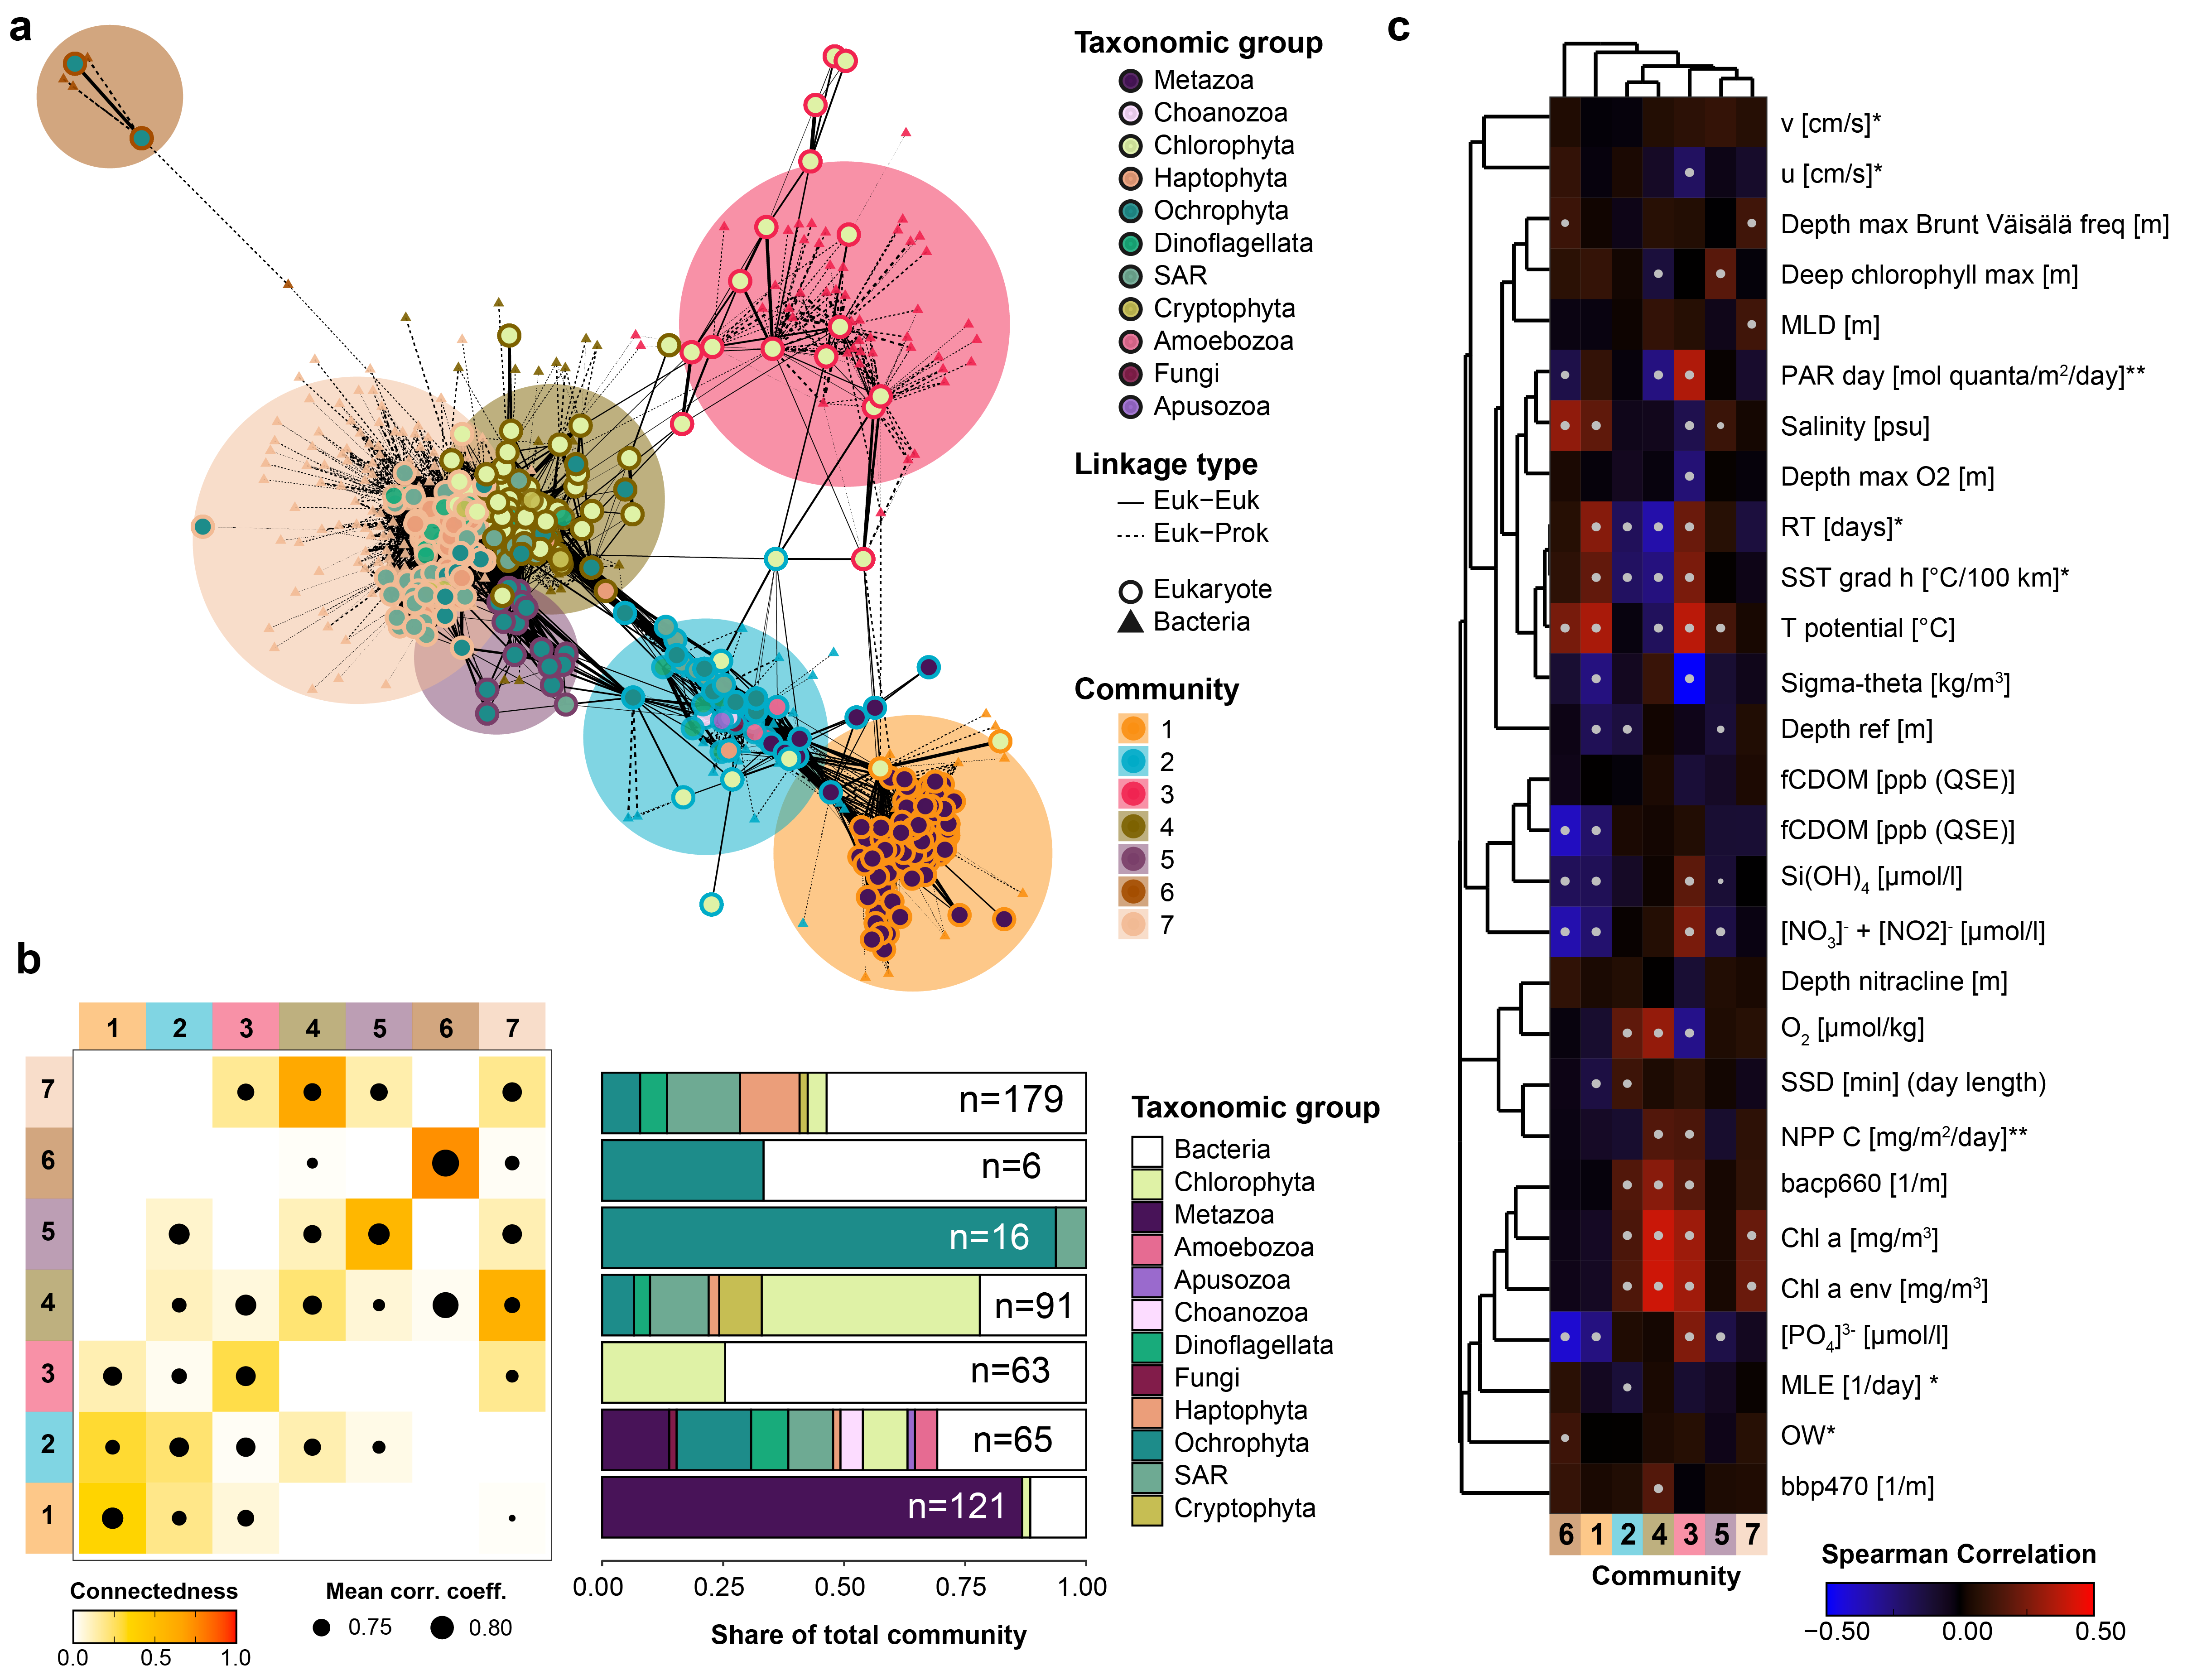
\includegraphics[width = \columnwidth]{figures/Figure6-networks.png}
    \caption{ \textbf{Distinct communities recovered from the TOPAZ MAGs.} a) A network analysis performed on the metagenomic abundance of all recovered eukaryotic and prokaryotic TOPAZ MAGs based on Spearman Correlation analysis, identifying 7 distinct communities (see materials and methods). A force-directed layout of the seven communities is shown with eukaryotes (circles) and bacteria (triangles). Only linkages between eukaryotes are visualized.   b) The connectedness and taxonomic composition of each community is depicted. Connectedness was calculated based on \Cref{eq:connectfinal}. c) A Spearman correlation between the summed metagenomic abundance of each community and environmental parameters from the sampling \citep{taraoceansconsortium2016ecoa}, modeled mesoscale physical features based on \citet{d_Ovidio_2010} (indicated with *), and averaged remote sensing products (indicated with **). Significant Spearman correlations, those with a Bonferroni adjusted $p<0.01$, are indicated with a dot on the heatmap.}    \label{fig:fig6-network}
\end{figure}

The co-retrieval of eukaryotic and prokaryotic MAGs from across the global ocean allows the unique opportunity to assess the biogeographical and ecological associations and potential co-occurrence of these organisms while also being able to infer likely function. To identify communities of associated organisms that co-occur across the surface ocean metagenomes, we performed a correlation clustering based on the abundances of the eukaryotic TOPAZ MAGS and the HQ-NR-TOPAZ MAGs (\Cref{fig:fig6-network} a). We employed a modularity optimization algorithm to the correlation analysis \cite{blondel2008fast} to identify distinct communities of co-occurring organisms. This approach identified seven distinct communities, which included 379 of the non-redundant TOPAZ MAGs (\Cref{fig:fig6-network} b). The communities were variably connected to each other, as defined by \Cref{eq:connectfinal}, with high connectedness among Communities 1, 2, and 3, and patchy connectedness among Communities 4-7 (\Cref{fig:fig6-network} b). Community 6 (the smallest of the communities, which consisted of a single Bacillariophyta TOPAZ MAG and five distinct \textit{Synechococcus} TOPAZ MAGs) had the highest inter-connectedness (0.733 connectedness), suggesting that members of this community co-occurred across samples with high fidelity. Moreover, this community was largely distinct from other communities and only shared significant connections to Community 7. The other six communities showed lesser degrees of inter-connectedness (range: $0.181-0.550$; mean: $0.365\pm0.204$), suggesting that they co-occur less consistently across samples. 

The seven communities that we identified based on metagenomic abundance correlations also significantly correlated with environmental factors, which consequently define the environmental niches where the communities were most abundant. Temperature was a primary factor defining the community correlations, significantly correlating with five of the seven communities. Community 4 correlated with colder temperatures and Communities, 1, 3, 5, and 6 correlated with warmer temperatures (\Cref{fig:fig6-network} c). In Community 4, we found significant positive correlations with chlorophyll and net primary productivity (Chla: $\rho=0.401$, $p=2.34e-35$, NPP: $\rho=0.166$, $p=1.28e-3$), while we found negative correlations with ``residence time'' ($\rho=-0.347$, $p=1.98e-14$), indicating a likely occurrence in newly formed eddies. Thus, Community 4 was largely found within colder, productive regions, and had enhanced metagenomic abundance in the Southern Ocean and the North Atlantic (\Cref{fig:network-map}). Community 4 was comprised of MAGs from Chlorophyta, Cryptophyta, Haptophyta, and Ochrophyta, the major groups containing primarily phototrophic eukaryotic microbes. 18 prokaryotic MAGs were also contained in this community, including both photosynthetic (Synechococcales) and non-photosynthetic lineages (e.g. Myxococcota and Planctomycetota). All told, this guild of MAGs comprises likely photosynthesizers often found in cold, but not necessarily nutrient-rich, environments. 

The four communities (1, 3, 5, and 6) that were positively correlated with temperature were distinguished by different correlations with nutrients and physical features. Communities 1 and 3 tended to be found in longer-lived eddies (according to the calculation by \cite{d2010fluid} as reported in the \textit{Tara} Oceans metadata \cite{taraoceansconsortium2016ecoa} as ``residence time'') (\Cref{fig:fig6-network} C; Community 1: $\rho=0.274$, $p=1.74e-8$, Community 3: $\rho=0.216$, $p=7.15e-5$). However, these two communities differed both in their association with nutrients and their taxonomic compositions. Community 1 was dominated by Metazoa and bacteria and correlated with oligotrophic conditions (nitrate and nitrite: $\rho=-0.234$, $p=1.21e-10$, phosphate: $\rho=-0.269$, $p=1.76e-14$, silica: $\rho=-0.190$, $p=1.02e-6$),  and was most abundant in the larger size fraction samples (20-2000 $\mu m$) (\Cref{fig:network-map}). By contrast, Community 3 was largely comprised of phototrophic chlorophytes and bacteria and was more likely to be found in high-nutrient environments (nitrate and nitrite: $\rho=0.230$, $p=3.04e-10$, phosphate: $\rho=-0.266$, $p=3.82e-14$, silica: $\rho=0.182$, $p=4.39e-6$), and was most abundant in smaller size fraction samples (0.8-20 $\mu m$), particularly around the tropics (\Cref{fig:network-map}). The other two warm-associated communities were comprised by SAR and bacteria (Community 5), and Ochrophyta and SAR (Community 6) (\Cref{fig:fig6-network} b). These communities were negatively correlated with nutrient concentrations (Community 5: nitrate and nitrite: $\rho=-0.140$, $p=3.17e-3$, phosphate: $\rho=-0.147$, $p=1.28e-3$, silica not significant; Community 6: nitrate and nitrite: $\rho=-0.355$, $p=1.68e-26$, phosphate: $\rho=-0.418$, $p=6.01e-38$, silica: $\rho=-0.187$, $p=1.92e-6$;), suggesting communities that thrive in oligotrophic regions.

While many of the communities recovered appeared to be driven largely by environmental forces, the genomic signatures of Community 1 members suggest that this community defined MAGs from both host and microbiome members. Community 1 was comprised primarily of Metazoa, specifically Hexanauplia, and bacterial MAGs (\Cref{fig:fig6-network} b). Many of the bacterial MAGs in Community 1 had genes that suggest adaptations to microaerophic niches such as those which might be experienced when living in close host association (e.g. high affinity oxygen cytochromes, and reductases) (\Cref{fig:community1-bact}). The bacterial MAGs in Community 1 could be broadly broken into two apparent functional types: those with larger genomes typical of copiotrophic bacteria and those with small genomes indicative potentially of reductive evolution.  The first group was comprised of MAGs from family Saprospiraceae in phylum Bacteriodota (n=2, 3.0 Mbp average genome size), the family UBA2386 in phylum Plactomycetota, which lacks cultured representatives (n=2, 3.3 Mbp), the order Opitutales in phylum Verrucomicrobiota (n=2, 3.4Mbp),  and the family Vibrionaceae (n=2, 4.5 Mbp) and order Pseudomonadales (n=2; 3.2 Mbp), both in phylum Gammaproteobacteria (\Cref{fig:community1-bact}). In addition to their relatively large size, the Saprospiraceae, Plactomycetota and Vibrionaceae MAGs were found to encode for  genes involved in the hydrolysis and utilization of various complex carbon sources including chitin and other carbohydrates (\Cref{fig:community1-bact}), such as those that might be shed or excreted by zooplankton such as copepods \citep{De_Corte_2017}.  By contrast, the second group of bacterial MAGs within Community 1 with smaller genomes, included MAGs from the Proteobacteria order Rickettsiales (n=3, 0.6-1.2 Mbp), Gammaproteobacteria family Francisellaceae (n=1, 1.2 Mbp), and the Bacteriodota family Amoebophilaceae (n=1; 0.8Mbp) \Cref{fig:community1-bact}).  The smaller genome sizes exhibited by these groups may be indicative of a genome streamlining which occurred with reductive evolution due to obligate or facultative symbiosis \citep{Giovannoni_2014}. Rickettsiales, Francisellaceae, and Amoebophilaceae all contain well-described obligate intracellular symbionts \citep{Santos_Garcia_2014, Darby_2007, Li_2021} and zoonotic pathogens \citep{ Celli_2013, Darby_2007}. 

\section*{Conclusion}
Sequence datasets are revolutionizing how we form new hypotheses and explore environments on the planet. Here, we demonstrated a critical advance in the recovery of MAGs from environmentally-relevant eukaryotic organisms with EukHeist. The retrieval and study of MAGs to study the role of microorganisms in environmentally significant biogeochemical cycling is promising; however the current lack of eukaryotic reference genomes and transcriptomes complicates our ability to interpret the eukaryotic component of the microbial community. We recovered 988 total eukaryotic MAGs, 485 of which were deemed highly complete. Our findings demonstrate that specific branches of the eukaryotic tree were more likely to be resolved at the MAG-level due to their smaller genome size, distribution in the water column, and biological complexity. A substantial portion of the recovered eukaryotic MAGs were distinct from existing sequenced representatives, demonstrating that these large-scale surveys are a critical step towards characterizing less-resolved branches of the eukaryotic tree of life. 

The continuing expansion of global-scale meta'omic surveys, such as BioGeoTraces \cite{Biller_2018} and Bio-GO-SHIP \citep{Ustick_2021}, highlights the importance of developing scalable and automated methods to enable more complete analysis of these data. Metagenomic pipelines that specifically integrate steps for handling eukaryotic biology, such as the EukHeist pipeline, are vital as eukaryotes are important members of microbial communities, ranging from the ocean, to soil \citep{bailly2007soil} and human- \citep{Luke__2015} and animal-associated \citep{Campo_2019} environments. The application of eukaryotic-sensitive methods such as EukHeist to other systems stands to greatly increase our understanding of the diversity and function of the "eukaryome".

\section*{Materials and Methods}

\subsection*{Data acquisition} The metagenomic and metatranscriptomic data corresponding to the size fractions dominated by eukaryotic organisms ranging from microbial eukaryotes and zooplankton ($0.8 -  2000 \mu m$) as originally published by \citet{Carradec2018global} were retrieved from European Molecular Biology Laboratory-European Bioinformatics Institute (EMBL-EBI) under the accession numbers PRJEB4352 (large size fraction metagenomic data) and PRJEB6603 (large size fraction metatranscriptomic data) on November 20, 2018. Only samples with paired end reads (forward and reverse) were used in the subsequent analyses (Supplementary Table 1). After an initial sample-to-sample comparison with sourmash (\texttt{sourmash compare -k 31 -scaled 10000}) \citep{Titus_Brown_2016} (\Cref{fig:sourmash}), it was determined that samples largely clustered by depth and size fraction. Samples were grouped for co-assembly by size fraction ($0.8 - 5 \mu m$, $5-20 \mu m$, $20-180 \mu m$, and $180-2000 \mu m$) as per \citet{Carradec2018global}, depth or sample type (surface (SRF), deep chlorophyll maximum (DCM), mesopelagic (MES), mixed surface sample (MIX), and filtered seawater (FSW)), and geographic location (Supplementary Table 1). In cases where a sample did not fall directly within one of the size classes, it was assigned to an existing size class based on the upper $\mu m$ limit of the sample. This grouping resulted in the combination of 824 cleaned, paired FASTQ files samples into 94 distinct co-assembly groups, which were used downstream for co-assembly (Supplementary Table 1). 

\subsection*{EukHeist pipeline for metagenome assembly and binning}The metagenomic analysis, assembly, binning, and all associated quality control steps were carried out with a bioinformatic pipeline, EukHeist, that enables user-guided analysis of stand-alone metagenomic or paired metagenomic and metatranscriptomic sequence data. EukHeist is a streamlined and scalable pipeline currently based on the Snakemake workflow engine \citep{Koster2012} that is configured to facilitate deployment on local HPC systems. \Cref{fig:flowchart} outlines the structure and outputs of the existing EukHeist pipeline. EukHeist is designed to retrieve and identify both eukaryotic and prokaryotic MAGs from large, metagenomic and metatranscriptomic datasets (\Cref{fig:flowchart}). EukHeist takes input of sequence meta-data, user-specified assembly pairings (co-assembly groups), and raw sequence files, and returns MAGs that are characterized as either likely eukaryotic or prokaryotic. 

Here, all raw sequences accessed from the EMBL-EBI were quality assessed with FastQC and MultiQC \citep{Andrews2010FastQC}. Sequences were trimmed using Trimmomatic (v. 0.36; parameters: \texttt{ILLUMINACLIP: 2:30:7, LEADING:2, TRAILING:2, SLIDINGWINDOW:4:2, MINLEN:50}) \citep{Bolger2014Trimmomatic}. Passing mate paired reads were maintained for assembly and downstream analyses. Quality trimmed reads co-assembled based on assembly groups (Supplementary Table 1) with MEGAHIT (v1.1.3, parameters: \texttt{k= 29,39,59,79,99,119}) \citep{Li2015MEGAHIT}. Basic statistics were assessed for all assemblies with Quast (v. 5.0.2) \citep{Gurevich_2013} (Supplementary Table 1). Cleaned reads from assembly-group-associated metagenomic and metatranscriptomic samples were mapped back against the assemblies with bwa mem (v.0.7.17) \citep{Li2010Fast}. The bwa-derived abundances were summarized with MetaBat2 (v. 2.12.1) script \texttt{jgi\_summarize\_bam\_contig\_depths} (with default parameters). The output contig abundance tables were used along with tetranucleotide frequencies to associate contigs into putative genomic bins using MetaBat2 (v. 2.12.1) \citep{Kang_2019}. The Snakemake profile used to conduct this analysis is available at \url{https://www.github.com/alexanderlabwhoi/tara-euk-metag}. A generalized version of the Snakemake pipeline (called EukHeist) that might be readily applied to other datasets is available at \url{https://www.github.com/alexanderlabwhoi/EukHeist}. MAGs here are subsequently named and referred to as \textbf{T}ara \textbf{O}ceans \textbf{P}article \textbf{A}ssociated MAGs (TOPAZ) and are individually named based on their assembly group (Supplementary Tables 2 and 3).

\subsection*{Identification of putative Eukaryotic MAGs} The binning process described above recovered a total of 16,385 putative bins. These bins were screened to identify high completion eukaryotic and prokaryotic bins. All bins were first screened for length, assuming that eukaryotic bins would likely be greater than 2.5Mbp in size (modeled off of the size of the smallest known eukaryotic genome, $\sim 2.3$Mbp \textit{Microsporidian Encephalitozoon intestinalis} \citep{Corradi2010complete}). Bins larger than 2.5Mbp were screened for relative eukaryotic content using EukRep \citep{West2018Genome-reconstruction}, a k-mer based strategy that estimates the likely domain-origin of metagenomic contigs. EukRep was used to classify the relative proportion of eukaryotic and prokaryotic content in each bin in a contig-by-contig manner. This approach identified 907 candidate eukaryotic bins that were greater than 2.5Mb in length and estimated to have more than 90\% eukaryotic content by length. Protein coding domains were predicted in all 907 putative eukaryotic bins using EukMetaSanity \citep{EukMS}. 

\subsection*{Protein prediction in Eukaryotic MAGs with EukMetaSanity} 
\paragraph{Taxonomy.} The MMseqs2 v12.113e3 \citep{Steinegger2017, Steinegger2018, Mirdita2019} \texttt{taxonomy} module (parameters: \texttt{-s 7 --min-seq-id 0.40 -c 0.3 --cov-mode 0}) was used to provide a first-pass taxonomic assignment of the input MAG for use in a downstream element of EukMetaSanity pipeline that requires an input NCBI taxon id or a taxonomic level (i.e. Order, Family, etc.). We created a custom database comprising both OrthoDB \citep{Kriventseva2018} and MMETSP \citep{Keeling2014} protein databases (OrthoDB-MMETSP) that integrates NCBI taxon ids. MMseqs2 was used to query each MAG against the OrthoDB-MMETSP database to identify a first-pass taxonomic assignment. The lowest common ancestor of top scoring hits was identified to provide taxonomic assignment to each candidate eukaryotic bin. The \texttt{taxonomyreport} module generates a taxon tree that includes the percent of MMseqs mappings that correspond to each taxonomic level. A taxonomic identifier and scientific name are selected to the strain level or when total mapping exceeds 8\%, whichever comes first. The assigned NCBI taxon id is retained for downstream analyses. 

\paragraph{Repeats identification.} RepeatModeler \citep{Flynn-RM, RepeatModeler} was used to provide \textit{ab initio} prediction of transposable elements, including short and long interspersed nuclear repeats, as well as other DNA transposons, small RNA, and satellite repeats. RepeatMasker \citep{RepeatMasker} was then used to hard-mask these identified regions, as well as any Family-level (as identified above) repeats from the DFam 3.2 database \citep{Flynn2020}. RepeatMasker commands \texttt{ProcessRepeats} (parameter: \texttt{-nolow}) and \texttt{rmOutToGff3} (parameter: \texttt{-nolow}) were used to output masked sequences (excluding low-complexity repeat DNA from the mask) as FASTA and gene-finding format (GFF3) files, respectively. 

\paragraph{\textit{Ab initio} prediction.}  GeneMark \citep{Lomsadze2005} was used to generate \textit{ab initio} gene predictions with the repeat-masked eukaryotic candidate bin sequences output from the prior step. The GeneMark subprogram ProtHint attempts to use Order-level proteins from OrthoDB-MMETSP database to generate intron splice-site predictions for \textit{ab initio} modeling using GeneMark EP  \citep{Bruna2020}. If ProtHint fails to generate predictions, then GeneMark will default to ES mode. Due to the fragmented nature of metagenomic assemblies, the prediction parameter stringency was drastically reduced relative to what is recommended for draft genome projects (parameters: \texttt{--min\_contig 500 --min\_contig\_in\_predict 500 --min\_gene\_in\_predict 100}). These parameters can be easily modified within the EukMetaSanity config file. GeneMark outputs predictions of protein coding sequences (CDS) and exon/intron structure as GFF3 files. 


\paragraph{Integrating protein evidence.} MetaEuk \citep{LevyKarin2020} was used to directly map the repeat-masked eukaryotic candidate bins sequences against proteins from the MMETSP \citep{Keeling2014, Johnson2018Re-assembly} and eukaryotes included in the OrthoDB v10 dataset \citep{Kriventseva2018}, hereafter referred to as the OrthoDB-MMETSP database. MetaEuk \texttt{easy-predict} (parameters: \texttt{--min-length 30 --metaeuk-eval 0.0001 -s 7 --cov-mode 0 -c 0.3 -e 100 --max-overlap 0}) used Order-level proteins to identify putative CDS and exon/intron structure. MetaEuk encodes this output as headers in FASTA sequences that are then parsed into GFF3 files. 

\paragraph{Merging final results.} GFF3 output from the previous \textit{ab initio} and MetaEuk protein evidence steps were input into Gffread \citep{Pertea2020} (parameters: \texttt{-G --merge}) to localize predictions from both lines of evidence into a single GFF3 output file.  Each locus was then merged together using a Python \citep{Python} script and the BioPython API \citep{BioPython} within EukMetaSanity. The set of \textit{ab initio} generated exons in each locus is used as a prediction of the underlying exon/intron structure of the gene locus to which it is assigned. If there are any protein-evidence-generated exons present at the same locus, and if the total numbers of exons predicted by each line of evidence have $\geq 70\%$ agreement, \textit{ab initio} generated exons lacking a corresponding protein-evidence-generated exon are removed (the first and last exon(s) of a locus are not removed). Conversely, any protein-evidence-generated exon present that lacks a corresponding \textit{ab initio} generated exon is added to the predicted exon/intron structure. The final gene structure for each locus is then processed into GFF3 and FASTA format.

\subsection*{Functional and taxonomic annotation of eukaryotic MAGs} 

Predicted proteins from EukMetaSanity were annotated for function against protein families in Pfam with PfamScan \citep{Finn2014Pfam} and KEGG using kofamscan \citep{Kanehisa_2019, Aramaki_2019} (Supplementary Tables 7 and 8). The relative completeness and contamination  of each putative Eukaryotic MAG was assessed based on protein content using BUSCO v 4.0.5 against the eukaryota\_odb10 gene set using default parameters \citep{Simao2015BUSCO} and EukCC v 0.2 using the EukCC database (created 22 October 2019 \citep{Saary2020Estimating}). Annotation and completeness assessment were carried out using a EukHeist-Annotate (\url{https://www.github.com/halexand/EukHeist-annotate}). EukCC \citep{Saary2020Estimating} was also used to calculate MAG completeness and contamination. The average completeness across groups increased in all cases with EukCC except for metazoans, which on average had a lower estimated completeness (\Cref{fig:eukcc}). 

The taxonomic affiliation of the high- and low-completion bins was estimated using MMSeqs taxonomy through EukMetaSanity and EUKulele \citep{Krinos2021EUKulele}, an annotation tool that takes a protein-consensus approach, leveraging a Last Common Ancestor (LCA) estimation of protein taxonomy, as well as MMSeqs2 taxonomy module \citep{Steinegger2017, Steinegger2018, Mirdita2019}. Taxonomic level estimation in EUKulele was assessed based on e-value derived best-hits, where percent id was used as a means of assessing taxonomic level, with the following cutoffs: species, >95\%; genus, 95-80\%; family, 80-65\%; order, 65-50\%; class, 50-30\% modeled off of Carradec et al. (2018). All MAGs were searched against the MarMetZoan combining the MarRef, MMETSP, and metazoan orthoDB databases \citep{Johnson2018Re-assembly, Keeling2014, Kriventseva2018, Klemetsen:2017fg}. This database is available for download through EUKulele. 

\subsection*{Phylogeny of eukaryotic MAGs} 
%A concatenated gene tree of the high-quality TOPAZ eukaryotic MAGs, the TARA MAGs (Delmont), and relevant select reference genomes and transcriptomes (MMETSP).
A total of 49 BUSCO proteins were found to be present across 80\% or more of the highly complete eukaryotic TOPAZ MAGs and were selected for the construction of the tree. Amino acid sequences from all genomes and transcriptomes of interest were collected and aligned individually using mafft (v7.471) (parameters: \texttt{--thread -8 –auto}) \citep{Katoh2013MAFFT}. Individual protein alignments were trimmed to remove sections of the alignment that were poorly aligned with trimAl (v1.4.rev15) (parameters: \texttt{-automated1}) \citep{Capella-Gutierrez2009trimAl}. Protein sequences were then concatenated and trimmed again with trimAl (parameters: \texttt{-automated1}). A final tree was then constructed using RAxML (v 8.2.12; parameters: \texttt{raxmlHPC-PTHREADS-SSE3 -T 16 -f a -m PROTGAMMAJTT -N 100 -p 42 -x 42}) \citep{Stamatakis2014RAxML}. The amino acid alignment and construction was controlled with a Snakemake workflow: \url{https://github.com/halexand/BUSCO-MAG-Phylogeny/}. Trees were visualized and finalized with iTOL \citep{Letunic2016Interactive}. 

\subsection*{Prokaryotic MAG assessment and analysis} 
The 15,478 bins that were not identified as putative eukaryotic bins based on length and EukRep metrics were screened to identify quality prokaryotic bins. The quality and phylogenetic-association of these bins was assessed with a modified version of MAGpy \citep{Stewart2019MAGpy}, which was altered to include taxonomic annotation with GTDB-TK v.0.3.2 \citep{Chaumeil_2019}. Bins were assessed based on single copy ortholog content with CheckM v \citep{Parks2015CheckM} to identify 2 different bin quality sets: 1) high-quality (HQ) prokaryotic bins (>90\% completeness, <5\% contamination), and 2) medium-quality (MQ) prokaryotic bins (90-75\% completeness, <10\% contamination). A total of 4022 prokaryotic MAGs met the above criteria. A final set of 2,407 non-redundant (NR) HQ-MQ MAGs were identified using dRep v2.6.2 \citep{Olm_2017}, which performs pairwise genome comparisons in two steps. First, a rapid primary algorithm, Mash v1.1.1 \citep{Ondov_2016} is applied. Genomes with Mash values equivalent to 90\% Average Nucleotide Identity (ANI) or higher were then compared with MUMmer v3.23 \citep{Mar_ais_2018}. Genomes with ANI $\geq99\%$ were considered to belong to the same cluster. The best representative MAGs were selected based on the dRep default scoring equation \citep{Olm_2017}. Out of the final set of 2,407 NR MAGs, 716 were HQ. The same pipeline was used to determine the HQ and MQ NR MAGs reconstructed from the \textit{Tara} Oceans metagenomes in previous studies \citep{Tully2018reconstruction, Parks2017Recovery, Delmont2018Nitrogen-fixing}. 

\subsection*{Phylogeny of bacterial non-redundant high-quality MAGs}
Only 5 out of the 716 HQ NR MAGs were found to belong to Archaea, thus only bacterial MAGs were used for the construction of the phylogenetic tree with GToTree v.1.4.10 \citep{Lee_2019} and the gene set (HMM file) for Bacteria (74 targets). GToTree pipeline uses Prodigal v2.6.3 \citep{Hyatt_2010} to retrieve the coding sequences in the genomes, and HMMER3 v3.2.1 \citep{Eddy_2011} to identify the target genes based on the provided HMM file. MUSCLE v3.8 \citep{Edgar_2004} was then used for the gene alignments, and Trimal v1.4  \citep{Capella_Gutierrez_2009} for trimming. The concatenated aligned is used for the tree constructions using FastTree v2.1 \citep{Price_2010}. Three genomes were excluded from the analysis due to having too few of the target genes. The tree was visualized using the Interactive Tree of Life (iToL) \citep{Letunic2016Interactive}.

\subsection*{Prokaryote MAG phylogeny comparison} 
A set of 8,644 microbial genomes were collected from the MarDB database \citep{Klemetsen:2017fg}(accessed 31 May 2018) encompassing the publicly available marine microbial genomes. Genomes were assessed using CheckM 
v1.1.1 \citep{Parks2015CheckM}(parameters: \texttt{lineage\_wf}) and genomes estimated to be <70\% complete or >10\% contamination were discarded. The remaining genomes (n = 5,878) were assessed using CompareM v0.0.23
(parameters: \texttt{aai\_wf}; \url{https://github.com/dparks1134/CompareM}) and near identical genomes were identified using a cutoff of $\geq 95\%$ average amino acid identity (AAI) with $\geq 85\%$ orthologous fraction (determined as one standard deviation from the average orthologous fraction for genomes with $97-100\%$ AAI).
Based on CheckM quality, the genome with the highest completion and/or lowest contamination were retained. From the remaining genomes (n = 3,843), all MAGs derived from the \textit{Tara} Oceans dataset, specifically from Tully et al. \citet{Tully2018reconstruction} and Parks et al. \citet{Parks2017Recovery}, were removed. The remaining genomes (n = 2,275) would be used to form the base of a phylogenetic tree representing the available genome diversity prior to the release of previous \textit{Tara} Oceans related MAG datasets \citet{Tully2018reconstruction, Parks2017Recovery, Delmont2018Nitrogen-fixing}, termed the ``neutral`` component of subsequent phylogenetic trees.

For the comparisons, phylogenetic trees were constructed using GToTree v1.4.7 \citep{Lee_2019} (default parameters; 25 Bacteria\_and\_Archaea markers). Any genome added to a tree that did not meet the default 50\% marker presence requirement was excluded from that tree. Five iterations of phylogenetic trees were constructed using the neutral genomes paired with each \textit{Tara} Oceans MAG dataset, the high-quality TOPAZ prokaryote MAGs, and the medium-quality TOPAZ prokaryote MAGs, individually, and two larger trees were constructed containing all neutral genomes and \textit{Tara} Oceans MAGs, with additions of either high- or medium-quality TOPAZ MAGs. Phylogenetic trees were assessed using genometreetk (parameter: \texttt{pd}; \url{https://github.com/dparks1134/GenomeTreeTk}) to determine the phylogenetic diversity (i.e., the total branch length traversed by a set of leaves) and phylogenetic gain (i.e., the additional branch length added by a set of leaves) \citep{Parks2017Recovery} for each set of MAGs compared against the neutral genomes and for the TOPAZ prokaryote MAGs compared against the neutral genomes and the other \textit{Tara} Oceans MAGs.

\subsection*{MAG abundance profiling} 

Raw reads from all metagenomic and metatranscriptomic samples were mapped against the eukaryotic and prokaryotic TOPAZ MAGs to estimate relative abundances with CoverM (v. 0.5.0; parameters: \texttt{-min-read-percent-identity 0.95 -min-read-aligned-percent 0.75  -min-covered-fraction 0 -contig-end-exclusion 75 -trim-min 0.05 -trim-max 0.95  -proper-pairs-only}; \url{https://github.com/wwood/CoverM}). The total number of reads mapped to each MAG was then used to calculate Reads Per Kilobase Million ($RPKM$), where for some MAG, $i$ :  $RPKM_i = {X_i}/{l_iN}10^9$, with $X =$ total number of reads recruiting to a MAG, $l =$ length of MAG in Kb, $N =$ total number of trimmed reads mapping to a sample in millions. We also calculated counts per million (CPM), a normalization of the RPKM to the sum of all RPKMs in a sample. CPM, a modification of transcripts per million (TPM) was first proposed by \citet{Wagner_2012} as an alternative to RPKM that reduces statistical bias. The metric has since been applied to metagenomics data, sometimes called GPM (genes per million) \citep{Gradoville_2017}. 

\subsection*{Nutritional modelling} 

To predict the trophic mode of the high quality TOPAZ eukaryotic MAGs (n=485), a Random Forest model \citep{Breiman_2001} was constructed and calibrated using the ranger \citep{Wright_2017} and tuneRanger packages in R \citep{tuneRanger}, respectively. The model was trained using KEGG Orthology (KO) annotations \citep{Kanehisa_2019} from a manually-curated reference trophic mode transcriptomic dataset consisting of the MMETSP \citep{Keeling2014} and EukProt \citep{Richter2020EukProt} (Supplementary Table 5). 644 of the transcriptomes in this reference dataset came from the MMETSP \citep{Keeling2014}, after 22 transcriptomes were removed due to low coverage of KEGG and Pfam annotations \citep{Finn2014Pfam}. The remaining 266 came from the EukProt database \citep{Richter2020EukProt}, after 162 were removed due having fewer than 500 present KOs. Nutritional strategy (phototrophy, heterotrophy, or mixotrophy) was assessed for each reference transcriptome individually based on the literature, 25\% of the combined reference transcriptomes were excluded from model training as testing data. 

A subset of KEGG Orthologs (KOs) that were predictive for trophic mode classification was determined computationally with the vita variable selection package in R \citep{Janitza_2016} (Supplementary Table 6), which was tested and justified by Degenhardt et al. \citet{Degenhardt_2017}. This process was carried out by the algorithm without regard to the predicted function of the KOs, but we found that many of these KOs were implicated in carbohydrate and energy metabolism, with preference for those KOs that differ strongly between heterotrophs and phototrophs (particularly for energy metabolism; \Cref{fig:ko-trophy}). The model was built using the selected KOs ($n=1787$ of a total 21585 KOs) with the 75\% of the combined database assigned as training data.

Additionally, we developed a secondary metric for assessing the extent of heterotrophy of a transcriptome or MAG. As opposed to the trinary classification scheme of the Random Forest model, this approach quantifies the extent that the MAG aligns with heterotrophic, phototrophic, or mixotrophic references by assigning a composite score. We calculated the likelihood of vita selected KOs used in the Random Forest model above to be present within heterotrophic, phototrophic, or mixotrophic reference transcriptomes. Three scores ($h$, $p$, $m$), one corresponding to each trophic mode, were hence calculated for each vita-selected  KO ($k$) ($n=1787$) (Supplementary Table 6). In  \Cref{eq:hks}, $K$ is the number of references the KO was present in for each trophic mode category, while $n$ is the total number of references available for each trophic mode category.

\begin{gather}\label{eq:hks}
    h_k = \mathbf{g}\left(\frac{K_\textrm{het}}{n_\textrm{het}}\right)\\
    p_k = \mathbf{g}\left(\frac{K_\textrm{photo}}{n_\textrm{photo}}\right)\\
    m_k = \mathbf{g}\left(\frac{K_\textrm{mixo}}{n_\textrm{mixo}}\right)\\
    \text{where, } \mathbf{g}(a) = \begin{cases}
       a & \textrm{if } a > 0.5 \\
       -(0.5-a) & \textrm{ otherwise} \label{eq:connectfinal}
    \end{cases} 
\end{gather}

If a given KO occurred in fewer than 50\% of the reference transcriptomes for a trophic mode, it was considered not to be characteristic of that trophic mode and as such the score, which we represent as the variable $a$, the ratio of the present KOs to the total for the subset of transcriptomes annotated some trophic mode (\Cref{eq:connectfinal}), was transformed ($-(0.5 - a),\ \text{if} \ a<0.5$), to reflect the absence without valuing absence over presence. In the test transcriptome dataset, the ratio-transformed scores were negated when a given KO was absent from the transcriptome. For instance, if a KO was absent from 90\% of reference transcriptomes assigned to heterotrophy ($a = 0.1$), and absent in the MAG or transcriptome being evaluated, it would receive a score of $h_k = -1 * (-(0.5-0.1)) = 0.4$ (\Cref{eq:hks}) for that KO. This reflects that the absence of the KO in the evaluated MAG or transcriptome aligned well with the high probability that the KO was absent among the reference transcriptomes.

The scores for all KOs selected by vita were then used to scale the presence/absence patterns observed across transcriptomes and MAGs. Thus, for each transcriptome or MAG a single score was calculated for each trophic mode heterotrophy ($H$), phototrophy ($P$), and mixotrophy ($M$) for all KOs present within the transcriptome or MAG ($K$):
  \begin{equation}\label{eq:sum}
  H = \sum_{k \in K} h_k \\ 
  \end{equation}
  \begin{equation}
    P = \sum_{k \in K} p_k \\
\end{equation}
  \begin{equation}
    M = \sum_{k \in K} m_k
\end{equation}

These calculated values can then be aggregated to a composite heterotrophy score ($H_{ind}$) (Supplementary Table 9). The score was computed as follows: 
\begin{equation}\label{eq:hind}
  H_{ind}=
    \begin{cases}
      -1^{(H-P)}\sqrt{(H-P)^2}, & \text{if}\ M-\max(H,P)<50, \\
      \frac{{}-1^{(H-P)}\sqrt{(H-P)^2}}{M}, & \text{if} \ M-\max(H,P) \geq 50
    \end{cases}
  \end{equation}
  
\subsection*{Ecological analysis of SAR and Dictyochophyceae MAGs}
24 highly-complete TOPAZ eukaryotic MAGs were subset to characterize the biogeography and putative trophic modes of \emph{Dictyochophyceae} and closely-related stramenopiles. MAGs included 11 \emph{Dictyochophyceae} MAGs and 13 MAGs belonging to a phylogenetically similar branch (Eukaryotic SAR; derived from the \texttt{MMSeqs} and \texttt{EUKulele} assignment). Metagenomic CPM abundance of MAGs was used to compare the biogeography and distribution of \emph{Dictyochophyceae} and closely-related stramenopile MAGs. MAGs were further classified based on trophic prediction and heterotrophy score. 

To investigate physiological potential, quality trimmed metatranscriptome reads were mapped using \texttt{Salmon} \cite{Patro2017Salmon} to the 24 MAGs. Comparison of of the putative metabolic capabilities of the predicted phototrophic versus heterotrophic MAGs was conducted in R3.6.1, where MAGs were clustered using the average distance between MAGs based on the presence and absence of known orthologs (KO annotations \citep{Kanehisa_2019}). Principle coordinate analysis of center log-ratio transformed TPM abundances of mapped reads from the smallest size fraction ($0.8 - 5.00 \mu m$) of all surface samples revealed the degree of overlap between \emph{Dictyochophyceae} and closely-related Stramenopile MAGs. Specific genes shared among all MAGs, shared across predicted trophic modes, and those vita selected KOs used in the trophic model (described above) were further targeted. All analyses described above are available at \url{ https://alexanderlabwhoi.github.io/2021-TOPAZ-MAG-Figures/}. 

\subsection*{Network Analysis} 

To identify co-occurring MAGs across the stations surveyed by \textit{Tara} Oceans, the CPM abundance of each highly-complete eukaryotic MAG ($>30\%$ BUSCO completeness) and each non-redundant, highly complete bacterial MAG was assessed at each station at all available depths and size fractions as described above. CPM was used because of the power of this metric for comparing samples directly: the sum of all CPM values per sample will be the same, as sequencing depth is accounted for after gene length. This makes it easier to compare the abundances of MAGs originally recovered from different sites \citep{Gradoville_2017}. A Spearman correlation matrix was generated to identify monotonic relationships between MAGs. Correlations were filtered based first on p-value, using the Šidák correction \citep{Sidak_1967}, a slightly less stringent metric than the Bonferroni correction. The Šidák correlation adjusts for multiple comparisons and is given by $p < 1-(1-\alpha)^{1/n}$, where $n$ is the total number of comparisons, and $\alpha$ is the significance value, in this case 0.05. We considered only those correlations within the 90th percentile of CPM correlations, thus correlations with absolute value less than 0.504 were removed from the analysis. Subsequently, we further filtered interactions to those with coefficient of correlation $>0.70$ for the construction of the network diagram. Because it was expected for several of the eukaryotic MAGs to be closely related (based on ANI), the relationships in the network were further filtered to exclude interactions between MAGs of exceedingly high similarity (having both $99\%$ ANI similarity and $>0.70$ coefficient of correlation in the network analysis) (Supplementary Table 12). ANI-based group members tended to have identical taxonomic classifications: only 2 of 94 clusters had different classifications at the order level per EUKulele (\Cref{fig:network-support}). 

We generated a network from this reduced set of labeled interactions (cut off at $>0.70$ coefficient of correlation, focusing on interactions between eukaryotes and prokaryotes or eukaryotes and eukaryotes, and using ANI-based clusters instead of MAG names when applicable) using \texttt{igraph} \citep{igraph,teamr} (Supplementary Table 11). Communities of highly associated MAGs were identified using a modularity optimization algorithm introduced in \cite{blondel2008fast} and implemented in \texttt{igraph} \citep{igraph}.

We assessed the connectedness within and between communities by calculating a connectedness metric as follows. For the connectedness within a community (one community to itself), we identified the number of ``dense'' connections by counting up the total number of links found between community members, regardless of how many times the particular MAG had been connected to its own community, and divided that number by the total possible ``dense'', meaning the number of connections which would exist if all community members were connected to all other community members. Between different communities, we defined connectedness by qualifying that a ``connection'' is made the first time each MAG from a given community is linked to another community, and calculated this quantity by dividing the number of realized links between community members by the maximum total size of the two involved communities (\Cref{fig:fig6-network} b; \Cref{eq:connect} - \Cref{eq:connectfinal}). 

\begin{gather}\label{eq:connect}
    C_{x,x} = \frac{\Sigma_{x=1}^{n_x} \Sigma_{y=1}^{n_y} f(x,x)}{\frac{n_x (n_{y-1})}{2}} \\
    C_{x,y} = \frac{\Sigma_{x=1}^{n_x} \Sigma_{y=x+1}^{n_y} f(x,y)}{\textrm{max}(n_x,n_y)} \\
    f(a,b) = \begin{cases}
       1 & \textrm{if } a \textrm{ and } b \textrm{ are connected} \\
       0 & \textrm{ otherwise} \label{eq:connectfinal}
    \end{cases} 
\end{gather}

We calculated Spearman correlation coefficients for the relationship between the abundance of communities between stations and several environmental parameters of interest from the \textit{Tara} Oceans metadata \citep{Pesant_2015, taraoceansconsortium2016ecoa} (\Cref{fig:fig6-network}). We considered the measured physical and chemical parameters, the modeled mesoscale physical oceanographic parameters, and averaged remote sensing products \citep{taraoceansconsortium2016ecoa, d_Ovidio_2010, Pesant_2015}. We adjusted the p-value of these comparisons using a Bonferroni adjustment within the statistics package in R \citep{teamr}. 

\subsection*{Data and code availability}
The eukaryotic and prokaryotic TOPAZ MAGs and Supplementary Tables 1-13 are available through the Open Science Framework (OSF) at \url{https://osf.io/gm564/} with the DOI: 10.17605/OSF.IO/GM564. EukHeist, which was used to recover the reported TOPAZ MAGs can be found at \url{https://github.com/AlexanderLabWHOI/EukHeist} and EukMetaSanity which was used for protein prediction in eukaryotic MAGs can be found at \url{https://github.com/cjneely10/EukMetaSanity}. Code used to generate the figures in this paper can be found at \url{https://github.com/AlexanderLabWHOI/2021-TOPAZ-MAG-Figures}. An interactive visualizer for the TOPAZ eukaryotic MAGs is available at \url{https://share.streamlit.io/cjneely10/tara-analysis/main/TARAVisualize/main.py} with source code at \url{https://github.com/cjneely10/TARA-Analysis}. 

\subsection*{Acknowledgements}
This research would not have been possible without the community driven efforts to provide open and freely available data by the \textit{Tara} Oceans Consortium. This research was supported by a National Science Foundation grant (NSF-OCE-1948025) to HA and a WHOI Independent Research and Development award to HA. AIK was supported by the Computational Science Graduate Fellowship (DOE; DE-SC0020347). BJT was supported by the Center for Dark Energy Biosphere Investigations (C-DEBI) through NSF-OCE-0939654. 

\subsection*{Author contributions statement}
HA and SKH conceived of and designed the study. HA carried out the assembly and binning. HA, AIK, SKH, MP, TR, and CJN, and BJT analyzed the data. HA and SKH wrote the manuscript with input from all authors. All authors edited and commented on the manuscript.

\section*{Ethics Declaration}
The authors declare no conflicts of interest.

\bibliographystyle{abbrvnat}
\bibliography{main}


\end{document}



